% !TEX encoding = utf8
% !TEX root = ../main.tex

% This content has been generated automatically from https://www.docx2latex.com/docx2latex_free and https://github.com/MartinoMensio/doc2latex_process_chapters 
% Consider editing the source Google Doc instead of this one!


\chapter{State of the Art}
\label{soa}

This section reports the related works on the topic of Conversational Agents. Having done some considerations about how the interaction among autonomous agents and humans was born and which social implication can rise, the discussion will focus on a classification of chatbots \ref{soaClassification}. Then the focus will go deep into technologies that can help building bots that can interact with the user through Natural Language \ref{soaNLU}. The last part will cover the topic of personalization \ref{soaPersonalization}.

\section{Chatbots and their classification}
\label{soaClassification}

Starting from the formulation of the Turing test, the problem of human-machine interaction has been analyzed and different solutions have been found. The terms that are commonly used for those kind of systems may vary (e.g \textit{chatbots}, \textit{conversational agents}, \textit{virtual assistants}), but the substance does not change: one interlocutor is not of human nature.

After the mobile-first wave that lead to a development of thousands of applications for devices that people pass the day with (e.g. smartphones, tablets, wearable devices and smart watches), is the transition to intelligent interactions that put the emphasis on natural and seamless interactions with automated systems. The interaction mean shifts from using well-designed and sometimes complicated interfaces made of buttons and paged procedures to textual or vocal dialogue. Asking questions naturally has many advantages with respect to traditional app interactions. The main one is that the user does not need to know how the specific app works, everyone knows how to communicate and in this case the system is coming towards the user to make the interaction more natural.

The evolution of these systems started long time ago, with first systems that were built to emulate a natural conversation, and has lead to today's virtual assistants that live on our smartphones and are ready to complete tasks for us.

The approaches that have been used have evolved through time to fit different needs and to overcome challenges that arise while developing such systems. The choice depends on the purpose of the bot. Bots can be designed to entertain the user in a conversation or can be designed to provide information on a specific field.

By firstly looking at the common applications of chatbots \ref{soaApplications} and existing classification in literature \ref{soaClassificationsExisting}, a classification will be done by considering the contents \ref{soaClassificationContents} and the approaches \ref{soaClassificationApproaches}. At the end the main challenges \ref{soaChallenges} are listed.

\subsection{Applications of chatbots}
\label{soaApplications}

Conversational Agents can be applied in all situations where there is a repetitive exchange of information with the user. The advantages can be both for users and companies.

On the side of the user, using applications can be quite frustrating sometimes. Every company has a different app that needs to be installed, configured and learnt to be used. The usage itself may result cumbersome. User interface forces to fill up information in a form-like structure. When finally you try to submit, you find out that you missed one required field. A conversational interface could simplify a lot this process, even though you are simply doing slot-filling and asking one input after the other.

Other advantages of conversational interfaces can be found when interacting with structured data whose criterion of navigability and search are not well known. Having an interlocutor that progressively helps refining our search, instead of filling a large form in an app, can help being more productive. Furthermore, voice commands can be used also without need to look and use hands, for situations where our attention is needed for other tasks.

From the point of view of the companies, the relation with the customer is the main channel to acquire and maintain customers. It is where the effort to understand users' needs should be maximum, and in many cases opting for offshore call centers may not be good and not very cheap. In these situations, having an automated responder could provide the service in the way you want in a scalable way.

The advantages of having those systems instead of dedicated people in \textbf{call centers} for customer support are many. First of all, the companies can support more customers because of the high scalability of those systems. For the majority of support requests, an automated response can be helpful. In case the system does not understand well the requests, a backup human solution can be called into action: in this way, also some very specific responses that were not designed in the requirements can be provided. The second major advantage for companies is that in this way they can have a set of responses more aligned with their guidelines. Establishing how the system should answer some types of questions once and for all, instead of having possible disinformation and misalignment of human employees. Eventually, when the automated system detects some difficulties due to the specificity of some issues with the user, an human responder can be used as backup solution: the chatbot will provide a first-line service and manage all the trivial interactions with the customers, using the human employees only when necessary.

Chatbots are also used in the field of \textbf{virtual assistants}. Using voice or text, we can interact with something that can quickly do things for us: adding events to the calendar, making phone calls and searching information on the Web. Virtual assistants provide a fast way to interact with the device, useful in situations where the users cannot interact in the visual way, for example while driving.

Also virtual assistants mainly fall into this category. On pre-determined domains (such as agenda management, meteo, sending messages) or also with external domains integrated by third-party apps (such as Alexa Skills,\footnote{\url{https://developer.amazon.com/alexa-skills-kit}} Cortana integration\footnote{\url{https://developer.microsoft.com/en-us/cortana}}) the assistant can help on a set of intents.

\subsection{Existing classifications}
\label{soaClassificationsExisting}

Since the fields of application and the possibilities are many, a search of classifications has been done in order to divide and find the main characteristics of this kind of bots.

Chatbots, in their larger definition, are software agents with whom you can carry a conversation. Accordingly to Franklin et Graesser~\cite{franklin1996agent}, there exist three main types of autonomous software agents that have different \textbf{objectives}: task-specific, entertainment and viruses, as can be seen in Figure~\ref{fig:franklinClassification}.

%%%%%%%%%%%%%%%%%%%% Figure/Image No: 1 starts here %%%%%%%%%%%%%%%%%%%%

\begin{figure}[!htbp]
    \centering
    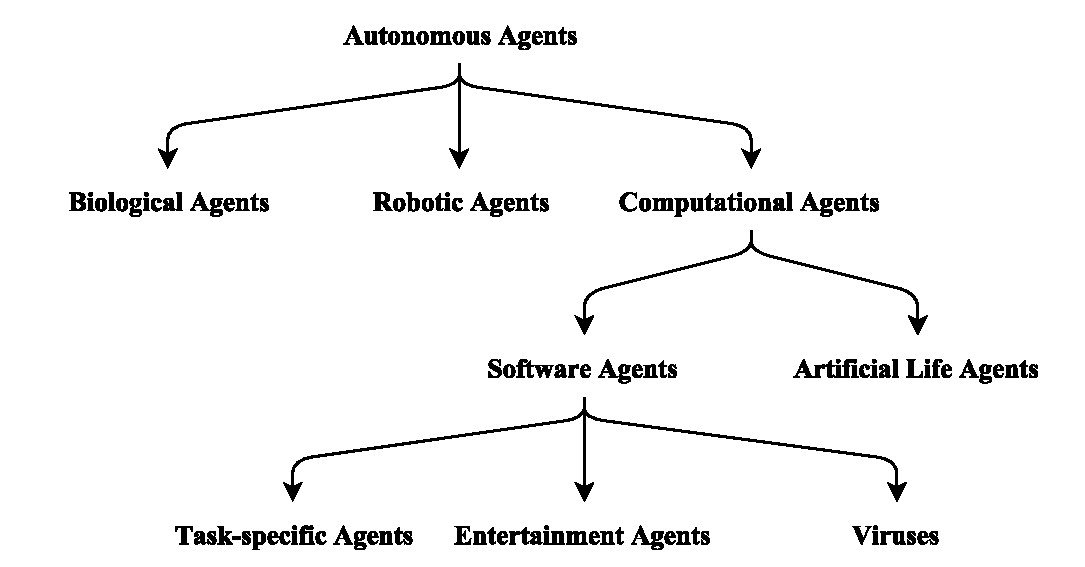
\includegraphics[max width=\linewidth,max height=8cm,keepaspectratio]{figures/franklinClassification}
    \caption{Natural Kinds Classification of Autonomous Agents in~\cite{franklin1996agent}}\label{fig:franklinClassification}
\end{figure}

Another division can be done by looking at the type of control mechanism: from rule-based systems that only follow handcrafted rules, to machine learning ones that learn dynamically from examples how to interact.

A very important characteristic to be considered when classifying conversational agents is the \textbf{initiative\footnote{ Jurafsky, D. (2017). Conversational Agents [PDF]. Retrieved from Stanford University course cs124 }}. With System Initiative only, the conversation is led by the bot and the user has only the possibility to say a finite set of things and cannot change directly the current state of the dialogue. It is the case when the user always replies to questions made by the bot, or when the only possibility of inputs is given by buttons. In dialogues between humans, the initiative usually shifts from one participant to another, and the same should apply in interactions with autonomous systems. For this reason, there exist mixed-initiative systems that try to take into consideration the user requests for tracking the dialogue state (and not imposing it).

Yet another division can be done by considering if the interaction scheme is single-turn (question followed by a response that only depends on the last question) or if the memory is required to perform a multi-turn dialogue. Multi-turn enables to refine searches and refer to entities previously mentioned, and are more natural than single-turn.

Other classifications that have been found are based on features such as believability and intelligence~\cite{isbister2002design}. Those features are reflected on how the user perceives the agent and are somehow similar to the goal of the imitation game: giving the illusion to talk to a person.

Given briefly those classification options, the choice has been to focus on two main dimensions for doing a classification: the first one (Section \ref{soaClassificationContents}) considers the contents of the dialogue, and is inspired by the objectives of Franklin et Graesser~\cite{franklin1996agent}. The second one (Section \ref{soaClassificationApproaches}) instead focuses on the approaches that are used.

\subsection{The information content}
\label{soaClassificationContents}

This first dimension considers the content of the conversation. Retaking the three objectives by Franklin et Graesser~\cite{franklin1996agent} (task-specific, entertainment, viruses) of autonomous software agents and removing the last one that is not inherent to conversational agents, the entertainment one is mapped to a generic chit-chat content (maintaining a general conversation with the user), while the task-specific one corresponds to domain specific knowledge (the bot provides it to the user acting as a natural language interface).

A third content type has been added to be able to categorize all those type of system that deal with different sources of information and combine them to provide rich answers. This may be called Encyclopedic Knowledge content, and the main ambition of those systems is to provide real answers to complex questions related to the world knowledge.

Those three main content types are explained in the following paragraphs, before going to discuss the existing approaches.

\subsubsection{Chit-chat}
The first type of content, that correspond to the native setting of the turing test because the goal is to entertain the user making him believe that the machine really understands the conversation, the history of chatbots is quite long.

The first chatbot ELIZA~\cite{weizenbaum1966eliza}, that was built in 1966, is of this kind. It was created mainly to demonstrate the superficiality of communications and the illusion to be understood by a system that is simply applying a set of pattern-matching rules and a substitution methodology.

ELIZA simulates a psychotherapist and, thanks to the trick of present again to the interlocutor some contents that have been previously mentioned, keeps the conversation without having an understanding of what really is said.\footnote{ ELIZA can be easily tested inside the text editor Emacs with the command doctor (meta-x doctor). } At the time when ELIZA came out, some people even attributed human-like feelings to the bot. A lot of other computer programs have been inspired by ELIZA. Even a markup language has been created to express the rules that drive the conversation (see AIML in \ref{aiml}).

A competition has been created to reward the progresses in this field: the Loebner Prize, an annual challenge that stands in the format of the Turing tests, but restricting the topics of conversation. Judges keep parallel conversations, one with a human and one with a computer program. Judges are chosen with the criterion that they $``$should respond naturally, as they would in a conversation with another person$"$ , in a way to avoid excessive sophistication. At the end the winner is the computer program that mostly convinced the judges (even without passing the Turing test). There are two more prizes in this competition: one is for the Turing test in text only interactions, the last one (the biggest one) is for passing the Turing test including visual and auditory inputs. This competition was first held in 1991, and with the years advancing the challenges have became more and more complex.

The Loebner Prize has been criticized by experts in the field because it rewards the usage of some tricks~\cite{shieber1994lessons}, pointing the focus on imitation instead of intelligence.

The commonly used tricks are~\cite{mauldin1994chatterbots}:

\begin{itemize}
	\item Let the conversation to be driven by the interlocutor. This works because most people like to talk about themselves and only want someone who listens;

	\item Give the illusion to be listening and understanding, by including substrings of the user input;

	\item Changing the topic when not understanding, that sometimes can be seen as paranoid;

	\item Simulated typing, delaying the responses.
\end{itemize}

The details of rule-based chatbots will be explained in more detail in \ref{soaRuleApproach}.

The evolution of chit-chat bots has recently evolved from a rule-based one to a generative approach. The key idea is to imitate existing conversations, and generate a response in a way that reflects both the training corpus and the current user turn (used as a stimulus). This approach, which will be discussed deeper in \ref{soaGenerativeApproach}, has its roots in using Statistical Machine Translation. The importance of the dialogue corpus, that dynamically establishes how the responses are generated, makes their availability a key element for a successful bot. For this reason these models are trained on few datasets publicly available: tweets, reddit discussions, ubuntu dialog corpus.

An example of this kind of systems is the mobile application Replika,\footnote{\url{https://replika.ai/}} that wants to provide a chat companion for its users. The conversation has no specific goals, and the system entertains the user with long discourses and games.

Focused on psychological support, an example of conversational system is Woebot.\footnote{\url{https://woebot.io/}} Entertaining the user with dialogues, it analyses the user mood and provides tips to feel better against depression and anxiety~\cite{fitzpatrick2017delivering}.

\subsubsection{Goal-oriented}
Another completely different type of bots is the one that provides a service on a restricted domain. It can be a natural language interface to a set of static Frequently Asked Questions, or can be linked to some dynamic content using some defined APIs. Those systems need to define the list of things they can do, and in some way map the user's requests to some actions.

Using those systems, the user should be aware of what the system can do and what cannot. Letting the user know that the bot he is interacting with can provide information only on the domain it is built for, should be a goal of the ideators. Responses for a little chit-chat conversation can also be added to the system, but they should be used only to avoid a general $``$\textit{I don't know}$"$  or $"$ \textit{I didn't understand}$"$ .

Those kind of bots can provide a more natural way of interacting with companies, both in the field of customer support and in search for information. The information can be statically defined as pairs of questions-answers. In this case the bot has to classify the user requests and provide the answer that mostly fits it. Or there can be some dynamic information that need to be extracted from the request. In this case, in addition to sentence classification, a parameter extraction needs to be performed. These tasks are the ones that this thesis will later focus on, and are the main part of the Natural Language Understanding process, which is described in \ref{soaNLUIntro} and analyzed in \ref{soaNLU}. The NLU approaches are quite handcrafted on the possible sentence types, and for this reason some more generative approaches are coming also in this field, inspired by the chit-chat domain. But what characterizes the conversational agents that provide this kind of content is the presence of a goal from the user: this is the reason that makes them called \textbf{goal oriented} agents.

\subsubsection{Knowledge-based}
As last type of chatbots, we can consider a richer version of the domain specific bot. Instead of limiting on a very restricted domain and predetermining the abilities with a static design of intents, this type of bots tries to provide a natural language interface towards a Knowledge Base. The fixed-structure intent based approach seems not to be optimal when the number of possible intents is very high and cannot be predetermined. If the system allows questions with a high level of complexity, requiring the linking of information, the number of intents quickly can explode.

Instead of doing a classification of sentences on some pre-defined intents, the goal of those systems is to transform the user sentence in a database query (for structured knowledge) or also to extract information from unstructured knowledge (such as documents expressed in natural language). This requires a strong relation between the Natural Language module and the Information Retrieval module. Structured knowledge can be composed of entities and relations between them. Information is in the form of RDF (Resource Description Framework) which have links to other entities with specific roles.

The sentences are analyzed using some parsers and are mapped to a set of linguistic patterns. After this translation (from human natural language to computer-understandable queries), the interrogation is performed using the content of a knowledge base. Those Question-Answering systems are actually very complex and involving different tasks and challenges~\cite{hoffner2017survey}.

A commonly used system that provides this kind of content is the Google Knowledge Graph, that explores the queries done on the search engine and provides linked information. Another example of them is the Wolfram Search, that can be asked questions like $``$\textit{who is the USA president?}$"$ . The focus here is not on managing complex dialogues, but understanding complex queries and exploring knowledge graphs.

There are however examples of encyclopedic knowledge systems that try to convey the conversational abilities of chit-chat dialogues empowering them with richer contents. This content ingestion is at the basis of the prototypes participating to the Alexa Prize.\footnote{\url{https://developer.amazon.com/alexaprize}} The goal that participants should try to achieve in this prize is to reach 20 minutes of dialogue with the user. Given a set of services (such as ASR, NLU, TTS), the teams have to design the dialogues and make it possible to carry on the conversation for the longest amount of time. Keeping such a long dialogue cannot be done by only providing simple responses using the tricks of ELIZA. Reasoning on topics requires having knowledge of them, so this kind of conversational agents are connected to knowledge bases.

\subsection{The approaches}
\label{soaClassificationApproaches}

The other dimension that is considered to make this classification is relative to the approach used. As will be seen shortly, bots require different stages (understanding, getting some information, answering) and different approaches can be applied to all of them.

As can be seen from the discussion on the content of the dialogue, there is an evolution of the approaches, leading to data-driven ones. The first wave of chatbot, as mentioned before, simply matched the input sentences with some keywords and responded in a way to make the conversation look natural. From this, a lot of other agents grew up with the same technique: pattern matching. With this approach, lots of bots have been built and even a specific markup language has been developed to express the patterns and link them to some responses.

More recent approaches instead tend to abandon the handcrafted rules towards an automatic learning from a dialogue corpus. This can be applied both to the part of natural language understanding (turn the user sentences into structured data) or also to the information retrieval and response generation.

We can do a classification of chatbot systems based on how much has to be specified and defined in a static way versus a dynamic approach that learns from the examples provided. This choice can be done in three main tasks: understanding, information retrieval, response generation. Each of them can have three levels of dynamicity: the first one is completely rule-based, the second one is mixed, usually presenting a dynamic categorization over pre-defined types, while the third one is completely dynamic. In the following Table~\ref{tab:approachCombination}, the levels are shown for each task.

%%%%%%%%%%%%%%%%%%%% Table No: 1 starts here %%%%%%%%%%%%%%%%%%%%

% !TEX encoding = utf8
% !TEX root = ../main.tex

\begin{table}
  \begin{tabularx}{\textwidth}{rLLL}
    \toprule
    \textbf{Dinamicity level} & \textbf{Understanding} & \textbf{Information retrieval} & \textbf{Response generation} \\
    \midrule
    0 & Pattern based (entities and intents) & None / Fixed data & Rule-based template \\
    \midrule
    1 & Machine Learning (entities and intents) & Fixed API & Dynamic template: retrieval based \\
    \midrule
    2 & Encoding (sentence embeddings) & Dynamic exploration & Generative \\
    \bottomrule
  \end{tabularx}
  \caption{The different approaches to Understanding, Information Retrieval and Response Generation}\label{tab:approachCombination}
\end{table}

The understanding task is the one related to turning the natural language sentences into something that can be understood by the machine: its output can be a pattern match for level 0, structured data for level 1 (NLU) or an encoded representation for level 2. 

The information retrieval task instead, if present, can use a fixed set of APIs or be more dynamic, interacting with information and their relations (graph knowledge bases).

Instead the response generation can be fully governed by handcrafted rules (e.g. if a set of conditions apply, say that). Or decide the template response from a finite set using statistical approaches (using some proximity measures like \textit{TF-IDF}, \textit{Word2Vec}, \textit{Skip-Thoughts}). Or being generative, with responses that are built on the fly by a seq2seq model.

%%%%%%%%%%%%%%%%%%%% Figure/Image No: 2 starts here %%%%%%%%%%%%%%%%%%%%

\begin{figure}[!htbp]
    \centering
    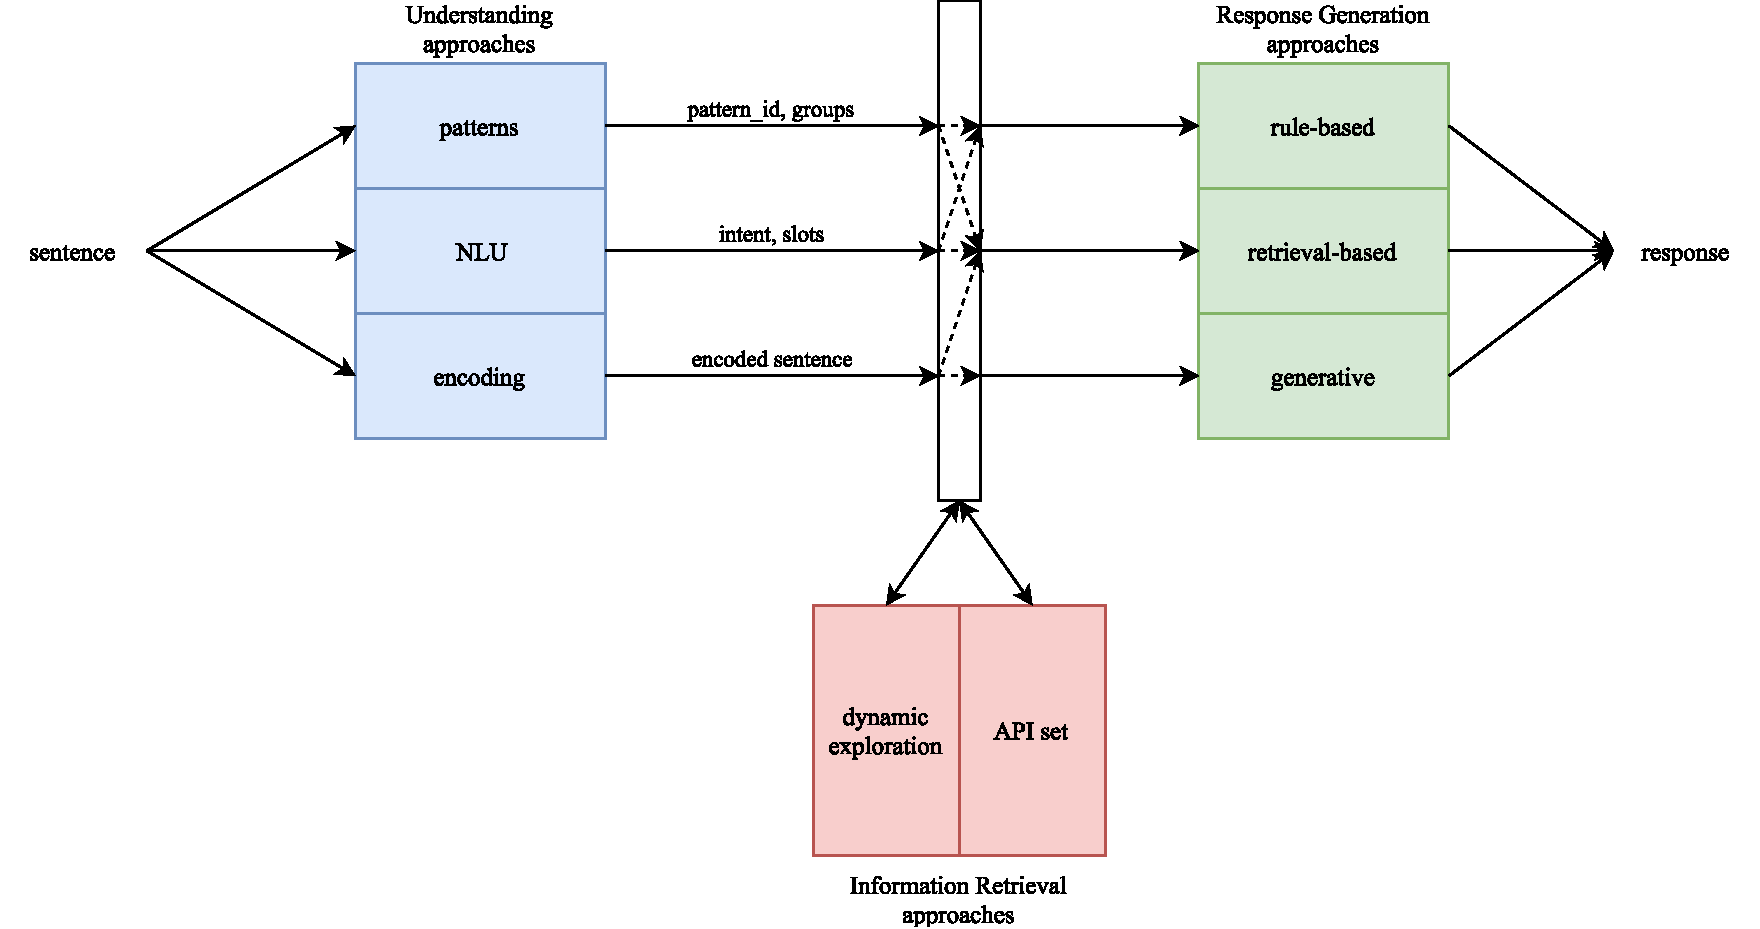
\includegraphics[max width=\linewidth,max height=8cm,keepaspectratio]{figures/approachesCombination}
    \caption{How the approaches for each task can be connected together}\label{fig:approachesCombination}
\end{figure}

The choices are not independent however, as can be seen from Figure~\ref{fig:approachesCombination}: since the tasks are put in a chain (first understanding, then retrieving the information and ultimately formulating a response), the approach chosen on the first stages has consequences on the following ones. Choosing to use ML instead of dynamic understanding precludes the possibility to have generative responses, because the user utterances will be categorized on a finite set of types (intent types) unless a hybrid understanding is performed (NLU to find the intent types with a parallel sequence-to-sequence model for chit-chat dialogues). For this reason and being the understanding stage the first one, the details on the approaches will be analyzed mainly on this first task, and for each level in it some details will be given on the possibilities for the other two choices.

The choice between those possibilities has to be done based on the available data (e.g. if transcripts of existing human conversations exist), and on the main information content the system will provide (see above, between chit-chat, domain-specific, knowledge-based) because the approach performance depend a lot on it. It is also necessary to keep in mind that complex dialogues actually can perform better if at dialog management level an handcrafted approach is kept. ML can help reconduct on sentence types, but actually structured topic dialogues need handcrafting. As of today, deductive (from rules) decision-taking in conversation gives better performances with respect to inductive (only learning from examples), because it gives more control to the designers of dialogues.\footnote{\url{https://developer.amazon.com/alexaprize}}

Moving the level of dynamicity higher, the \textbf{complexity} moves from handcrafting very specific features, that can be very specific to the domain of application and therefore provides a solution that difficulty can be ported to new domains, to the complexity of the approach itself. The transition usually is towards approaches that involve machine learning techniques like neural networks: the engineering of those networks is quite complex with respect to writing patterns to cover a set of sentences. In addition, also more computing power is required to run those heavy systems.

Changing the selected approach (especially on the understanding and generation processes) also has consequences on the additional work that has to be done to port the agent to \textbf{other languages}. A rule-based understanding is highly coupled with the used language. Using NLU reduces a lot this dependence because instead of manually deciding how to categorize the sentences, the system will find automatically how to do that even in another language, if the appropriate annotated training examples are provided and if the network structure itself is sufficiently language independent. As will be described in the NLU chapter, using features of words that are more related to their meaning (contextual and semantic, following the $``$distributional semantics$"$  concept) instead of their grammatical role, helps generalizing and being less dependent on the selected language (see usage of word embeddings and how they can be easily generated for any language).

Summing up, a more dynamic, end-to-end approach has an higher complexity but leads to easily adaptable solutions, in terms of new domains and new languages.

\subsubsection{Rule-based}
\label{soaRuleApproach}

This approach has both the understanding part and the response generation specified as rules. It was firstly used for chit-chat systems, and the number of rules can be quite big. Those rules can define theirself a response or can refer to other rules in order to reduce the amount of different actions. However this strategy is not very good because a lot of rules must be written in order to span all the possible variations of sentences. Moreover, since the majority of the work is to write those rules, and the rules highly depend on the language analyzed, this approach can hardly be applied on different languages and the process of migration from one to another requires the rewriting of the whole set of rules.

Chit-chat systems historically do not use knowledge bases to provide responses. The information that they provide is statically written as part of the  system background.

This approach was firstly used by ELIZA~\cite{weizenbaum1966eliza}. Then, when used by ALICE, an extended version of ELIZA, there has been the release of AIML, that is the markup language used for expressing the rules. With the release of AIML, lots of implementations of chatbots used this approach.

\label{aiml}

\textbf{AIML} stands for Artificial Intelligence Markup Language and is a language that describes how the bot replies to certain inputs. Inputs are evaluated against a set of patterns and the best matching (category) is chosen. The actions performed by the category can be a simple response or can also set the values of state variables and invoke other categories. Those rules determine together the classification of the sentences and the response generation.

A rule (in the AIML jargon is called category) is made up of a pattern and a template. As can be seen in~\ref{fig:aimlExample}, the pattern is responsible to identify the sentences that activate the rule, while the template is the part that manages the response: a template can be both a sentence that will be sent to the user or can be a redirection towards another rule (\textit{srai} rules). In addition to those two elements, some actions to manage the state of the conversation can be added: variables can be set and read to to conditionally activate rules.

%%%%%%%%%%%%%%%%%%%% Figure/Image No: 3 starts here %%%%%%%%%%%%%%%%%%%%

\begin{figure}[!htbp]
    \centering
    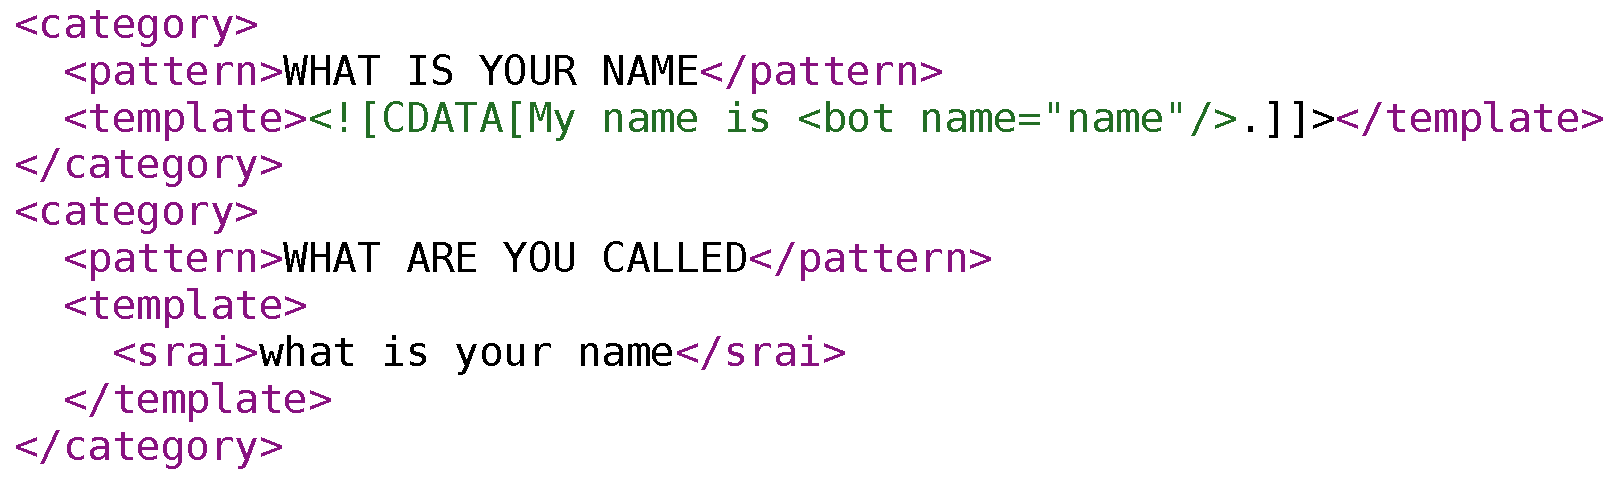
\includegraphics[max width=\linewidth,max height=8cm,keepaspectratio]{figures/aimlExample}
    \caption{An example of the rule-based AIML}\label{fig:aimlExample}
\end{figure}

While writing those rules can be quite easy, the problem is that a lot of them must be written to manage the variations on the natural language. In fact, the strategy used for managing the development cycle of bots empowered by AIML is a cyclical process: starting with a model with some rules, the system is tested against a group of test users collecting the interactions; at the end of the test session, the logs are analyzed and the developers modify and add rules to provide suitable responses. This process is called \textbf{targeting}. The developer role can be separated from the role of tester or testers can be given privileges to modify the rules on their own.

The disadvantages of using AIML are many. First of all, being a rule based system, a big set of rules need to be built and so a big fraction of time is spent analyzing the possible variation of the sentences instead of leaving it for more important tasks such as focusing on the data available. A lot of rules are also needed to perform reduction on other rules. Those additional rules make very difficult to understand what is wrong when multiple reduction rules have been applied. Other problems come when the sentences contain complex queries. In this situation, it is possible that more parameters need to be extracted from a single sentence, and since every pattern can contain a maximum of one wild character some tricks must be used.

AIML is used on bots based on ALICE. Being the markup language released under GNU GPL license, a lot of open source tools exist, only requiring the developers to produce a set of AIML rules. Even online services exist that can be used to deploy an AIML bot in very few steps (for example pandorabots\footnote{\url{https://home.pandorabots.com/en/}}).

Also considering that AIML was born for generic chit-chat systems and the Loebner Prize, it has been used also in domain specific bots. For example, to provide answers to Frequently Asked Questions in the domain of student support in Universities~\cite{ghose2013toward}. The information contained in the FAQ are relative to admissions and courses information. The AIML rules for managing conversations on these topics have been added to a base ALICE bot, and a change in the state transition management has been done in order to make the conversation stay on the desired topics, using weighted transitions that make the bot prefer to stay on the university domain. This system has been tested on students, establishing some evaluations on their satisfaction and also on the topic switching rate, in order to have some measures on the state transition management.

Other examples of rule-based systems are bots that manage the interaction with the user by only providing \textbf{buttons}. In this way, the dialogue is completely managed by the bot and the interlocutor can only decide on a finite set of choices at every turn. This is a very unnatural dialogue scheme, where the initiative belongs completely to the bot. A lot of bots today belong to this category, because in this way the dialogues are strongly reliable and the state of conversation can be tracked and managed easily without unexpected utterances. About the information retrieval, those bots usually interact with a fixed set of APIs (as most domain-specific bots do).

\subsubsection{NLU}
\label{soaNLUIntro}

Another approach that can be used for the understanding task, instead of manually matching sentences with patterns, is to have a Natural Language Understanding engine that performs this classification in a smarter way. In this approach, instead of building rules and analyzing the structure of the sentence in order to span the different variation of sentences that should be grouped together, the objective is to have a classifier that can be trained to make this task automatically using machine learning techniques (feeding training examples, letting the internal parameters to be adjusted automatically to obtain the desired outputs).

Natural Language Understanding applies only to the task of understanding the sentences (turn natural language sentences into structured data), and not to the response generation. NLU is composed of two subtasks: sentence classification, also called intent detection, that finds for each input sentence a predetermined type that expresses what the user wants to communicate or ask; slot filling, also called entity extraction, that is responsible to obtain from sentences some parameters that have been previously defined in their type.

This approach is born for domain specific bots and responds to a problem that is inborn to this kind of bots: exists a big difference between the natural language and the information with fixed structure stored in knowledge bases. Using Natural Language Understanding techniques, an intermediate representation can be built starting from the sentences in natural language and from this representation, composed of intent and entities, it is easier to interface with the fixed structure information that are usually reachable using some statically defined APIs (information retrieval) and also manage the state of the dialogue, recording which intents and entities have occurred (dialogue manager).

NLU can also be used when the dialogue manager is not statically defined, but is trained to provide the correct responses and call the right APIs over a predefined set. In this solution, there are not rules defining how to track the state of the conversation, because they are inferred from the training corpus. This technique, for example, is used by the open source company RASA,\footnote{\url{https://rasa.ai/products/rasa-core/}} that provides a model that not only takes care of NLU (handling intents and entities), but also can manage a dynamic state tracking. Based on a fixed set of patterns provided by the developer and actions (that may call external APIs), the state tracker can be trained both by providing dialogue examples or by doing online learning (asking for feedback after every turn) for a quick annotation of new corpora.

\subsubsection{Encoder-Generative models}
\label{soaGenerativeApproach}

Going further with automation techniques that learn from examples, if the management of the state of the dialogue and the information retrieval and the response generation are managed without writing static rules, the approach is said to be generative. Using this approach removes the intermediate point of contact between natural language and rule-based systems that is used in NLU systems. Everything is trained together in a end-to-end fashion: from the input sentences to the output sentences.

This approach was born in the chit-chat domain and has its strength when combined with a huge corpus of dialogues. Given the dialogues, which are sequences of sentences said by different actors, the system is trained to generate the next sentence given the current dialogue history.

The first implementation of this strategy was trained on tweets~\cite{ritter2011data}, but other works have been trained on Ubuntu Dialogue Corpus~\cite{lowe2015ubuntu} and many other datasets.

The technology used is the one that is used to provide translations, with some modifications. The model for the generation is trained on the corpus and learns how to generate the next sentence from the previous ones with an encoder-decoder structure. This structure, as will be seen applied for slot tagging in \ref{soaSeq2Seq}, uses LSTM cells, that can capture features of sequences adaptively using the memory capabilities of their recurrent nature. The encoder network (can be seen as the understanding part) collects the useful features while the decoder, given an initial state from the encoder and given a stimulus, begins the generation of the new sentence and stops when appropriate.

A even more complex approach is the one described in~\cite{serban2016building} that uses a hierarchical RNN: the lower level is applied on words, both in the encoder and the decoder, while a coarse-grained RNN applied on the sentences is used to model the topic propagation over the turns.

The main advantage of this kind of approach is that responses are generated completely in automatic way and thanks to LSTM cells can contain elements that were previously mentioned in the conversation. Being generative, they always produce an output even when the inputs are very different to the ones used in the training phase. This can be seen as good generalization ability, but can result in the generation of unpredictable and strange sentences, even when huge corpora are used for training. Grammatical errors can also be generated in the output sentences if no post processing checks are done.

To overcome those problems, reinforcement learning strategies can be applied, in order to learn in an online setting also from the dialogues that occur at runtime. This is a good strategy in general, but it can lead to some unwanted effects of polarity of the responses if there is not a supervision: the example of Microsoft Tay, that after 16 hours on Twitter was shut down because of the offensive tweets that was generating.\footnote{\url{https://www.washingtonpost.com/news/the-intersect/wp/2016/03/24/the-internet-turned-tay-microsofts-fun-millennial-ai-bot-into-a-genocidal-maniac/}}

Having a model trained on a wide variety of dialogues also rises the problem of the coherence of the responses: it is easy that, without filtering and post-processing the responses, the bot replies in different ways to questions inherent to the same topic. For this reason a persona-based model can be built in order to consider also some more inputs to the generator of the responses, that can model some features of the speaker, such as background information and speaking style~\cite{li2016persona}. Those features can be encoded into distributed embeddings and be provided to the generator both in the training and in the inference time.

Another common problem of this approach is that it tends to generate commonplace responses, because it is trained to maximize the likelihood of the output for the given input. It is like providing an average response that fits the current input. A proposed solution to reduce this effect is to use Maximum Mutual Information as objective function in the neural model. This will try $``$\textit{to take into account not only the dependency of responses on messages, but also the inverse, the likelihood that a message will be provided to a given response}$"$~\cite{li2015diversity}. Using this solution, a clear decrease in the proportion of generic responses can be observed on the outputs.

This generative approach has shown good results for non-specific task dialogues, because the goal is simply to continue the dialogue and there is no need to introduce some task-specific information.

As an example of this approach in action, Google Smart Reply applies it to generate short email responses that can selected and completed. The implementation takes in account the incoming email to generate responses that may be used to replay~\cite{kannan2016smart}.

In the field of domain specific bots, usually the responses are not generated completely from sequence-to-sequence models. The approaches usually make use of templates that can be chosen by rules or by a dynamic classifier. But in some way templates are always used to provide the answers to domain-specific questions.

The dynamism can also reach higher levels on the information retrieval task, without requiring fixed APIs but allowing simple key-value data storage to be queried in natural language: this approach has been proposed by Eric and Mannings~\cite{eric2017key}.

\subsection{The challenges}
\label{soaChallenges}

For the different contents and approaches that have been analyzed, different challenges arise with bots that should provide some kind of valuable content.

The most important point is to classify the user sentences and to reconduct them to a set of questions that have a response by design. This challenge of \textbf{understanding} the user is made up of two components: one is relative to the natural language understanding of the current sentence, while the other one is relative to the contextualization of the current sentence in the environment of the dialogue. While talking, humans tend to refer to previously mentioned things, and the understanding of sentences is often difficult without placing it into its \textbf{context}. Some approaches to solve this problem are explained in the section \ref{soaInteractionContext}, explaining the concept of multi-turn and dialogue tracking.

Another challenge that arises, especially on generative approaches, is the \textbf{coherence} of the sentences that are said. Since the training of those models is done on dialogues between multiple users with different visions and different behaviour, it may be difficult to establish a coherent personality of the bot. This issue is not present if the approach chosen makes the response generation in a static way: in this case it is sufficient to keep a coherent personality among the people writing the response templates.

Another big issue is how to deal with \textbf{unexpected questions}, for which a response has not been prepared. This problem is present in rule-based approaches, in NLU-based bots and even in generative approaches.

The next section will investigate the Natural Language techniques that are used for domain specific bots, focusing on the tasks of intent recognition \ref{soaIntent} and slot filling \ref{soaSeq2Seq} and how to manage a dialogue in a multi-turn environment \ref{soaInteractionContext}.

\section{Natural Language Understanding}
\label{soaNLU}

As introduced previously, NLU is the process of turning sentences into structured information. Two asks are involved:intent classification and slot filling. Usually those tasks are performed in statistical way, not applying a static set of rules as was done with AIML and similars. Natural Language Understanding belongs to the Natural Language Processing (NLP) family whose components are involved in text processing in very different ways.

Starting from the easiest NLP component, tokenizers are part of this family. The role of a tokenizer is to split texts into tokens that correspond to words and also punctuation (if punctuation is relevant for the current problem, or can be removed by the tokenizer).

Other important components of NLP are Part-Of-Speech recognizer and Dependency Parser, that are responsible to parse (this term is also used when elaborating source code; some approaches can be taken from source code parsing, but usually the natural language grammar is more complex and ambiguous and is better analyzed by statistical parsing~\cite{ballesteros2015improved}) the sentence and individuate the grammatical roles of the words.

Another commonly used component of NLP is the Lemmatizer: its role is to reconduct to the base form all the words that derive from others. This is used to reduce the cardinality of vocabularies and simplify some tasks, for example finding the topic of the conversation.

Another thing that is done using NLP is Named Entity Recognition: this finds occurrences in the text of some entities that belong to some types: common types are Person, Organization, Country, Location, Date, Time, Numbers, Currencies. This component usually mixes an approach based on POS combining them with a knowledge base that enumerates in some way what belongs to each entity type. The Slot Filling task is quite similar to NER, and the differences will be analyzed soon. The NER can have some complications when the talker refers to previously mentioned entities by using explicit signs (such as pronouns or definite nominals) or implicit references (such as ellipsis): this is the non trivial problem of \textit{coreference resolution}, that is analyzed in \ref{soaCoreference}.

Other components are more focused on the sentence as a whole: Sentiment Analysis that tells if a sentence is positive negative or neutral, Summarization, Sentence Classification to find topic or complexity level for example. The intent detection task can be put in this last group.

For this work we are interested mainly in two very specific tasks (intent classification and slot filling that are described soon) that usually are denoted by the Natural Language Understanding label. The other NLP tasks (syntactical analysis, POS tagging) are not main interests here, however some of them, such as sentiment analysis, can be used to detect the mood of the writer, as will be discussed in the personalization section \ref{soaPersonalization}.

\subsection{Goals}
As mentioned before, from the sentences NLU wants to:

\begin{itemize}
	\item Classify the intent (what the user wants, against a set of predefined ones);

	\item Extract the entities mentioned (we may want to care about only a specific set of entity types that are relevant to the abilities of the bot). This task is somewhere called slot filling, because the words that we want to extract may also not be entities. $``$The slot filling task is to search a document collection to fill in values for predefined slots (attributes) for a given entity.$"$  Furthermore, slots in a sentence can be designed to have a role (in order to be able to discriminate between multiple instances of the same type of entity). This feature is not present in the Named Entity Recognition task because the objective is only to recognize the entities, not to give them a role as a parameter in a programming language. For this reason the name of this task can be both $``$slot filling$"$  and $``$entity extraction$"$  with preference for the first one that gives more the idea of roles, while $``$named entity recognition$"$  is quite unappropriate.
\end{itemize}

For example, for the sentence $``$is Turin a supported city?$"$  we may want to categorize it as a question that asks if a city is supported (this is the intent) and extract the word $``$\textit{Torino}$"$  that is the city the user is looking for (this is a slot that corresponds to an entity of type CITY or simply LOCATION depending on the granularity of entities defined).

The first task corresponds to a classification of the user sentences to decide what is the intention of the user. Since a bot is usually designed to answer to different types of questions, this stage is responsible for finding the type of question. The slot filling task instead is a process that annotates some parts of the input sentences with the name of the corresponding slot. A slot can be thought as a field in an online form. While the intent represents the type of question, the slots of a sentence are values that the bot must be able to extract from the sentences because they are used as parameters for the application logic.

For both the goals, different approaches are described in dedicated subsections: the intent classification related ones are analyzed in \ref{soaIntent} while the slot filling ones in \ref{soaSeq2Seq}.

Once the intent and the slots have been analyzed on the current sentence, we can have some rules at the application level that can put some constraints. For example, for a certain type of question, one or more slots can be compulsory. In this case, the conversation should make the user provides the values by prompting him some questions. These types of constraint make the interaction model more complex and require an analysis over multiple user and machine turns, as will be seen in Section \ref{soaInteractionContext}.

The two tasks can be done independently, but some recent studies (like~\cite{guo2014joint} and~\cite{liu2016attention}) have shown that there can be benefits if they are performed together.

\subsection{Recurrent Neural Networks}
This section contains a description of the different structures of neural networks that have reached the State of the Art condition and have been described in literature.

A neural network approach can be used for the tasks of slot filling and intent detection. The first thing that needs to be done is to point out what are the inputs and outputs of the system. Once defined the inputs and outputs, we can think of a component that implements the desired functionalities. The inputs to the network are the words contained in the sentence and the outputs are the intent label (for the intent classification task) and the slot labels (for the slot filling task).

As slot labels, the slot names can be used directly but, in order to better handle multi-word slots, a commonly used format is the IOB introduced in~\cite{ramshaw1999text}, where the O indicates $``$other$"$ , the B is the beginning of a slot and the I is the label associated with a word that continues the slot of the previous word. The IOB labels are prepended to the slot name.

An example of inputs and expected outputs, showing the IOB annotation scheme, is represented in Figure~\ref{fig:iob}.

%%%%%%%%%%%%%%%%%%%% Figure/Image No: 4 starts here %%%%%%%%%%%%%%%%%%%%

\begin{figure}[!htbp]
    \centering
    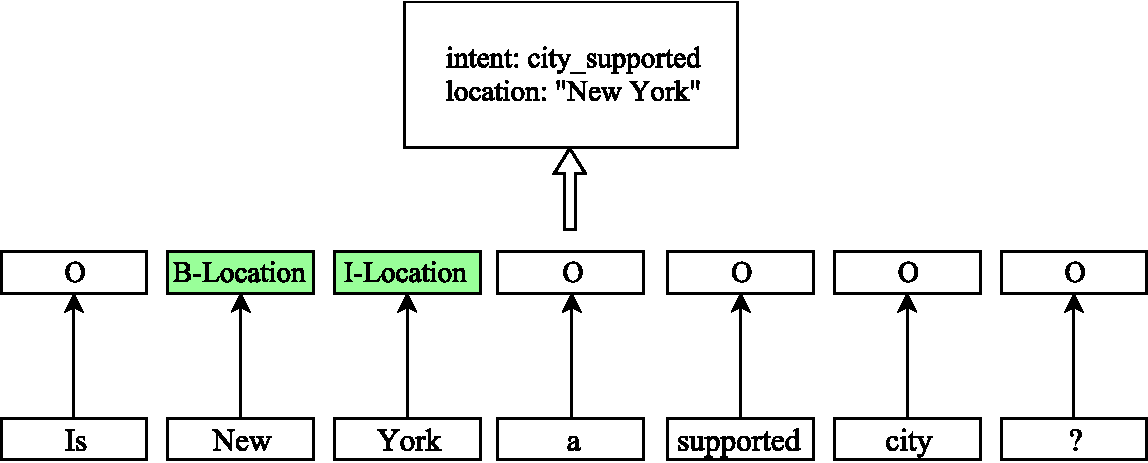
\includegraphics[max width=\linewidth,max height=8cm,keepaspectratio]{figures/iob}
    \caption{The Inside Out Beginning annotation scheme}\label{fig:iob}
\end{figure}

Instead of using simple feed-forward networks, a lot of studies make use of networks with recurrent components. The core idea behind RNN is to make use of sequential information. In feed-forward networks, the assumption is that each input-output pair is independent from the others. For RNN, the recurrence stays in performing the same task for every element of the sequence, making the output depending on the previous steps. This idea can be seen as the RNN having memory that keeps information from the past iterations. Specifically on the ability of remember and use in the correct way their memory, a lot of studies have been done to develop particular cells (a cell is the basic building block for RNNs).

%%%%%%%%%%%%%%%%%%%% Figure/Image No: 5 starts here %%%%%%%%%%%%%%%%%%%%

\begin{figure}[!htbp]
    \centering
    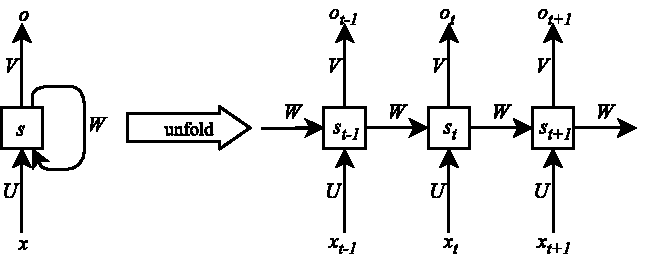
\includegraphics[max width=\linewidth,max height=8cm,keepaspectratio]{figures/rnnUnfold}
    \caption{The temporal unfolding operation on a simple RNN structure}\label{fig:rnnUnfold}
\end{figure}

A recurrent cell is a type of cell that takes as input also its previous output. Those types of neural networks have been designed for problems where the order of inputs matters, and the length of input sequence can vary. For example, they are commonly used with sequence of words, characters, frames in a video and their goodness stands in modeling features that belong to the sequence. Unlike feed-forward nets, that consider the fixed set of inputs to generate the outputs, the recurrent nets are applied in different timesteps to elements belonging to a sequence and, thanks to the loops of their cells, retain information from previous timesteps and the output depends on them too.

Since the same network (and cells) are used in different timesteps, the analysis of RNN is usually performed on the unfolded version of the network (see Figure~\ref{fig:rnnUnfold}): the single elements are repeated different times (one for each timestep) and the looping links are now going from the element in the previous time to the next time. In this way, a recurrent network is transformed into a multi-layer feedforward network, but keeping the same weights on the unfolded elements that generate from the same recurrent cell.

The unfolding operation sometimes is also called unrolling because of the similarity to the loop unrolling.\footnote{\url{https://en.wikipedia.org/wiki/Loop\_unrolling}}

\subsubsection{Backpropagation}
Backpropagation is the algorithm used in neural networks to update the weights, that is used also for the training of recurrent networks, with a slight modification.

The goal of the backpropagation training algorithm is to modify the weights of a neural network in order to minimize the error of the network outputs compared to some expected output in response to corresponding inputs. It is a supervised learning algorithm that allows the network to be corrected with regard to the specific errors made.

The general algorithm is as follows:

\begin{itemize}
	\item Present a training input pattern and propagate it through the network to get an output;

	\item Compare the predicted outputs to the expected outputs and calculate the error;

	\item Calculate the derivatives of the error with respect to the network weights;

	\item Adjust the weights to minimize the error;

	\item Repeat with other training samples.
\end{itemize}

In this way the Neural Network, which is a combination of layers with tunable parameters, learns to predict the expected output of the training samples. The goodness of the network is to obtain correct outputs also for reasonably similar samples that were not seen in training time.

With RNNs the training mode is very similar. The name of the modified algorithm is BackPropagation Through Time (BPTT)~\cite{werbos1990backpropagation} and is basically the standard algorithm applied on the temporally-unfolded version of the network. The only difference is that, since the layers correspond to different timesteps of the same cell, the weight updates in each instance are summed together. In other words, the temporally-unfolded neural network is a deep neural network with shared weights.\footnote{\url{http://www.wildml.com/2015/10/recurrent-neural-networks-tutorial-part-3-backpropagation-through-time-and-vanishing-gradients/}}

As can be see in Figure~\ref{fig:bptt}, the loss function in backpropagation for each observed error (the difference between the true value and the predicted one, denoted with  \( E \) ) affects the current and previous timesteps with partial derivatives. For example, if we want to consider the gradient of the error  \( E_{2} \) with respect to the inputs  \( x_{2} \) ,  \( x_{1} \) and  \( x_{0} \)  we can apply the chain rule:

 \(  \frac{ \partial E_{2}}{ \partial x_{2}}=\frac{ \partial E_{2}}{ \partial s_{2}}\cdot \frac{ \partial s_{2}}{ \partial x_{2}} \) 

 \(  \frac{ \partial E_{2}}{ \partial x_{1}}=\frac{ \partial E_{2}}{ \partial s_{2}}\cdot \frac{ \partial s_{2}}{ \partial s_{1}}\cdot \frac{ \partial s_{1}}{ \partial x_{1}} \) 

 \(  \frac{ \partial E_{2}}{ \partial x_{0}}=\frac{ \partial E_{2}}{ \partial s_{2}}\cdot \frac{ \partial s_{2}}{ \partial s_{1}}\cdot \frac{ \partial s_{1}}{ \partial s_{0}}\cdot \frac{ \partial s_{0}}{ \partial x_{0}} \) 

%%%%%%%%%%%%%%%%%%%% Figure/Image No: 6 starts here %%%%%%%%%%%%%%%%%%%%

\begin{figure}[!htbp]
    \centering
    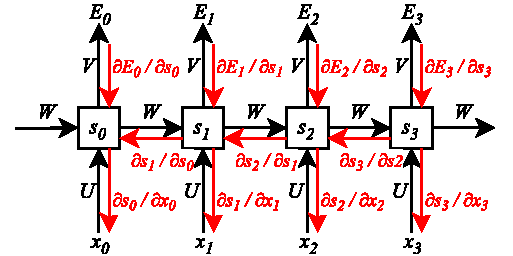
\includegraphics[max width=\linewidth,max height=8cm,keepaspectratio]{figures/bptt}
    \caption{The Backpropagation Through Time: how the errors are propagated}\label{fig:bptt}
\end{figure}

\subsection{Cell types}
This paragraph describes the  cell types used in this thesis. Such cells are the basic units used for the network architectures explained successively. As a layer in feedforward NN is composed of neurons, a layer in a RNN is composed of a recurrent cell. The cell holds the matrix parameters to compute outputs and next state given the current state and current input.

\subsubsection{Simple RNN}
The simplest recurrent cell type is a block with two inputs and two outputs. As can be seen in Figure~\ref{fig:simpleRNN}, one input is the actual input at the current timestep while the other one comes from the previous timestep (or from initialization on the first time). The cell produces an output ( \( y_{t} \) ) that can be passed to the next layers of computation (recurrent or not) or be used as a probability distribution passing through a \textit{softmax}. For the next timestep the cell also produces the current state ( \( h_{t} \) ) that is used on the looping connection; the state has the same value as the output, and the different name is given only to to put the emphasis on the different destinations for each one of them.

%%%%%%%%%%%%%%%%%%%% Figure/Image No: 7 starts here %%%%%%%%%%%%%%%%%%%%

\begin{figure}[!htbp]
    \centering
    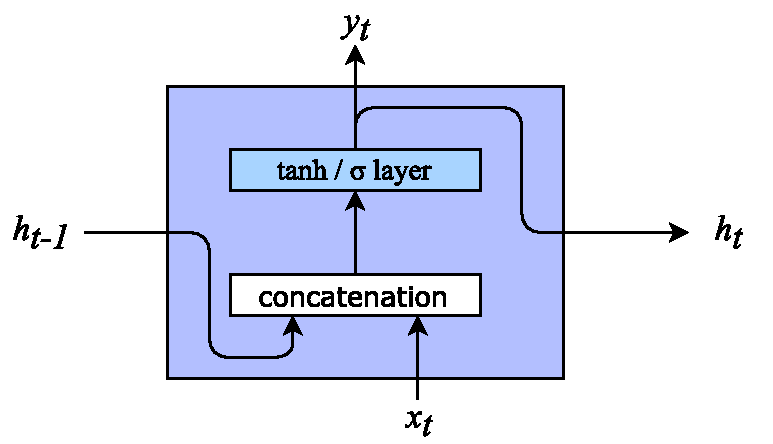
\includegraphics[max width=\linewidth,max height=8cm,keepaspectratio]{figures/simpleRNN}
    \caption{A simple RNN with a single layer inside}\label{fig:simpleRNN}
\end{figure}

The two inputs are concatenated and passed through a single feed-forward layer that corresponds to a linear transformation plus a non-linear function (e.g.  \( tanh \) ,  \(  \sigma  \) ). The next state is computed as  \( h_{t}=tanh \left( W\cdot  \left[ h_{t-1}, x_{t} \right]  + b \right)  \)  where the notation of square brackets denotes the concatenation operation, and  \( W \)  and  \( b \)  are respectively weights and biases.

Since the same cell is applied many times in time, and the recurrence loop feeds back the output as inputs, there can be easily two kinds of problem due to the fact that the weight matrix coefficients are multiplied at each timestep:

\begin{itemize}
	\item Exploding gradient: if some coefficients are greater than 1, the output values can become soon very big, making the network insensible to new inputs because is in some way saturated. The solution to this problem is using some non-linear function that limits the values not to be over the value of 1;

	\item Vanishing gradient: if some coefficients are near to 0, the network will quickly forget previous inputs and the output will not depend on them.
\end{itemize}

This can also be seen in the formulation of BPTT. There are two factors that can affect the magnitude of gradients - the weights and the activation functions (or more precisely, their derivatives) that the gradient passes through. If either of these factors is smaller than 1, then the gradients may vanish in time; if larger than 1, then explosion might happen. For example, the  \( tanh \)  derivative is smaller than 1 for all inputs except 0; sigmoid  \(  \sigma  \)  has even lower values because it is always less than  \( 0.25 \) .

Those problems have the same origin: the simple RNN is not able to manage long-term dependencies. This problem has been analyzed in detail by~\cite{bengio1994learning},~\cite{hochreiter1998vanishing} and other types of cells have been proposed.

\subsubsection{LSTM}
LSTM~\cite{hochreiter1997long} is a solution that came out in 1997 in which a more complex cell is considered. The main idea is to have some gates that decide how much of the previous cell state to keep, and how much of the current input to consider for the calculation of the current state and current output.

%%%%%%%%%%%%%%%%%%%% Figure/Image No: 8 starts here %%%%%%%%%%%%%%%%%%%%

\begin{figure}[!htbp]
    \centering
    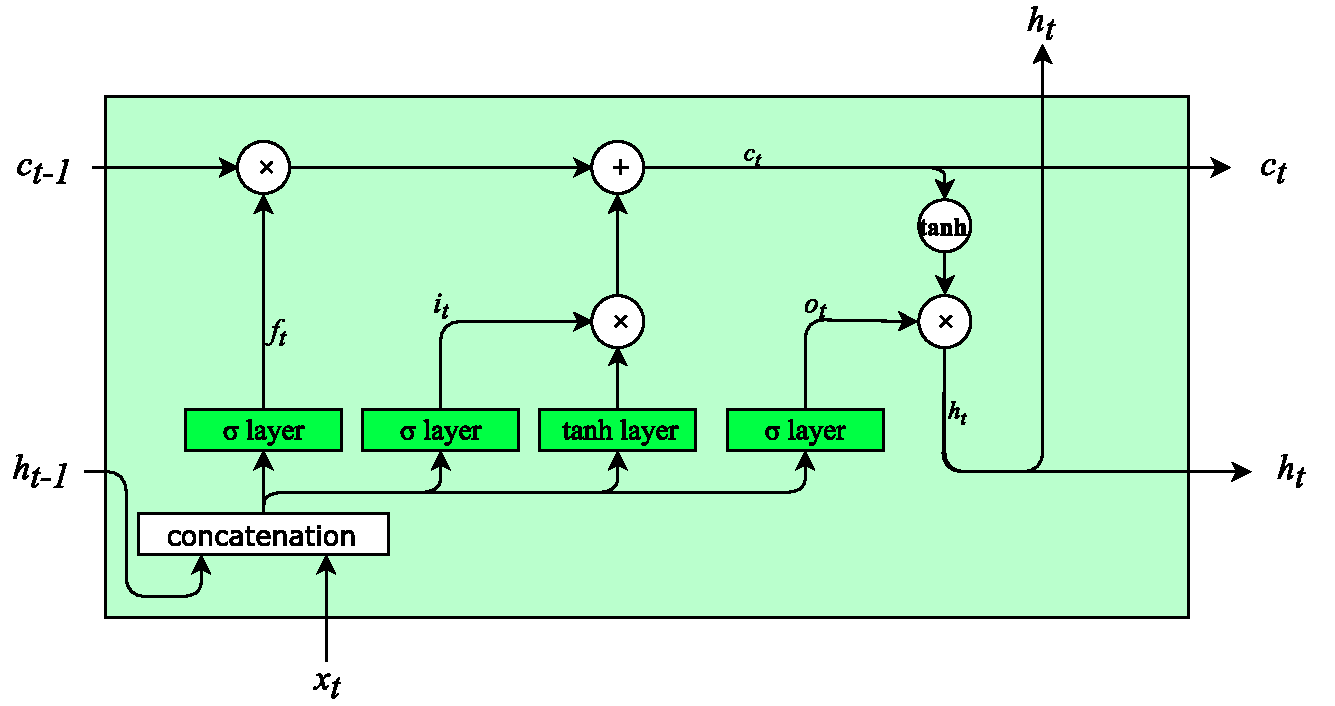
\includegraphics[max width=\linewidth,max height=8cm,keepaspectratio]{figures/LSTM}
    \caption{The Long Short-Term Memory cell proposed in~\cite{hochreiter1997long}}\label{fig:LSTM}
\end{figure}

In addition to the simple RNN cell, we can see in Figure~\ref{fig:LSTM} that three more \textit{gates} are added:

\begin{itemize}
	\item Forget gate  \( f_{t} \) :\ decides how much of the previous hidden state to keep.   \( f_{t}=tanh \left( W_{f}\cdot  \left[ h_{t-1}, x_{t} \right]  + b_{f} \right)  \) 

	\item Input gate  \( i_{t} \) : decides how much of the current input to consider.  \( i_{t}=tanh \left( W_{i}\cdot  \left[ h_{t-1}, x_{t} \right]  + b_{i} \right)  \) 

	\item Output gate  \( o_{t} \) : decides how much of the hidden state is exposed to the output.  \( o_{t}=tanh \left( W_{o}\cdot  \left[ h_{t-1}, x_{t} \right]  + b_{o} \right)  \) 
\end{itemize}

All those gates are implemented with single layer feedforward networks. This type of RNN is able to manage better the long-term dependencies, at the expenses of having four times the parameters. But with sufficient training examples, the network is able to learn how to output the correct values and how to mix the different inputs.

Many implementation\ exist of this cell, the most common is the basic LSTM that is shown in  Figure~\ref{fig:LSTM}, but variations exist (with peephole connections, or other variations on the gates\footnote{\url{http://colah.github.io/posts/2015-08-Understanding-LSTMs/}}).

The gates are combined with the previous cell state  \( c_{t-1} \)  and hidden state  \( h_{t-1} \)  in the following way: the input gates  \( i_{t} \) are used to scale the outputs of a  \( tanh \)  layer (the layer that was used in simple RNN) and produce the state update candidate  \( \hat c_{t} \) . Then the forget gates  \( f_{t} \)  decide how much to keep of the previous cell state  \( c_{t-1} \)  and produce the new state  \( c_{t}=f_{t}\cdot c_{t-1}+i_{t}\cdot \hat c_{t} \) . At the end the new hidden state is computed using the output gate:  \( h_{t}=o_{t}\cdot tanh \left( c_{t} \right)  \) .

The LSTM addresses the problem of vanishing gradients very specifically. In the recurrency of the LSTM, the activation function is the identity function (the addition from  \( c_{t-1} \)  to  \( c_{t} \) ) with a derivative of  \( 1.0 \) . So, the backpropagated gradient neither vanishes or explodes when passing through, but it remains constant. The effective weight of the recurrency is equal to the forget gate activation. So, if the forget gate is on (activation close to  \( 1.0 \) ), then the gradient does not vanish. Since the forget gate activation is never greater than  \( 1.0 \) , the gradient cannot explode either.

\subsubsection{GRU}
Later studies~\cite{cho2014learning} have proposed a new type of cell/unit GRU that has only two gates: reset gate and update gate that adaptively control how much each hidden unit remembers or forgets while processing a sequence. The hidden state and the state cell are merged together and therefore the output gate is no more required.

%%%%%%%%%%%%%%%%%%%% Figure/Image No: 9 starts here %%%%%%%%%%%%%%%%%%%%

\begin{figure}[!htbp]
    \centering
    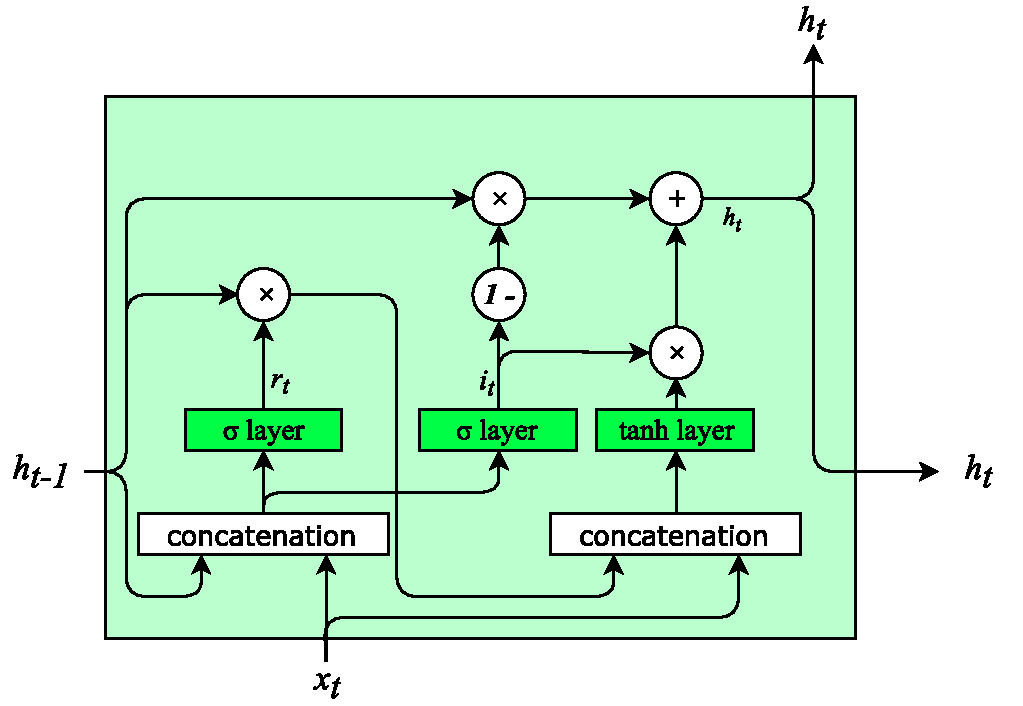
\includegraphics[max width=\linewidth,max height=8cm,keepaspectratio]{figures/GRU}
    \caption{The Gated Recurrent Unit cell porposed in~\cite{cho2014learning}}\label{fig:GRU}
\end{figure}

The advantage of this type of element with respect to LSTM is that less parameters are used.

Figure~\ref{fig:GRU} shows the internal composition of the cell. The analysis of how the internal layers are connected can be done by taking as reference the simple RNN with only the  \( tanh \) layer. GRU firstly adds the reset gate  \( r_{t} \) that modulates how much of the previous state  \( h_{t-1} \) is passed to the basic  \( tanh \) layer. The other gate, the update one  \( i_{t} \) decides the weighting between the basic  \( tanh \) output and the previous state  \( h_{t-1} \) : if the values are close to  \( 1 \) , the cell works similarly as a simple RNN that suffers from long-dependencies irrelevance (fading gradients), but as the values of this gate decrease the behavior of the cell tends to keep its state unchanged.

It is important to notice that this cell has only one state vector: no distinction between visible  \( c_{t} \) and hidden  \( h_{t} \) , the architecture is simpler.

Being more recent, less studies have used them, but from the performance point of view, they seem to be of the same order of LSTM (like~\cite{jozefowicz2015empirical} and~\cite{chung2014empirical}).

\subsection{Word embeddings}
\label{soaWordEmbeddings}

Now that the bases of recurrent networks have been described, let us focus on a very important point: inputs. The choice of the inputs to the neural network is very important and can affect a lot its performances.

It might seem that we already have the inputs to the Neural Network: sentences. Sentences are made up of words and we would like to use those words as inputs to the classifier network.

But since all neural networks only work with numbers, there must be a layer at the beginning that, given the input words, transforms them in numerical form.

The most simple and naive approach is to consider the $``$one-hot$"$  vector of the words. This representation is an array with length corresponding to the length of the input dictionary and contains values that are all zeros except for the one whose index corresponds to the index of the word in the vocabulary. In other words, a dictionary is built and the representation of the i-th word in the dictionary is an array with a single non-zero value on the i-th value. This is straightforward to implement, but has some problems because highly depends on the input dictionary: the length of one-hot vectors is the same as the length of the dictionary. Any network following this representations will have a big problem: different words, with similar meanings, will be completely different so any parameter that can be learnt on one words will not be applicable to a similar word. This approach cannot work with words that are not contained in the training set.

Other solutions may employ techniques like stemming or lemmatization, that try to reduce the vocabulary by stripping out word suffixes and reconduce words to their roots. Stemming, applies brutally some rules to remove the suffixes, while lemmatization extracts the lemma with more powerful and studied rules. However those techniques remove information that could in some way be useful, and make human language very rich.

A better approach is to use a representation of words that considers semantics and syntactic information. The hypothesis behind this method is the Distributional Semantics~\cite{sahlgren2008distributional}:\ words that appear in the same context (the context is there defined as the surrounding words) are considered similar, because somehow they can be exchanged the one for the other since they appear in similar contexts. With this hypothesis, each word is mapped to a dense real vector with a fixed dimension,  where the values are optimized to represent the semantical distribution of the corresponding words. Their dimension is a lot smaller than the size of the input dictionary. The word embeddings are usually pre-trained on large corpora of unlabeled data (for example Wikipedia\footnote{\url{https://dumps.wikimedia.org/}} or CommonCrawl\footnote{\url{http://statmt.org/ngrams/}}).

With these vectors it is possible to perform different things:

\begin{itemize}
	\item Find neighbors and compute the similarity of words;

	\item Visualization on 2D plane~\cite{maaten2008visualizing};

	\item Mathematical operations with words that represent analogies of relationships among words: this can be measured with the so called \textit{analogy test~\cite{mikolov2013linguistic}}.
\end{itemize}

Using word embeddings as inputs to the neural network has the advantages~\cite{bengio2003neural}:

\begin{itemize}
	\item Reduced size of input arrays, no $``$curse of dimensionality$"$ ;

	\item Semantic and syntactic similarities of words are considered.
\end{itemize}

The embeddings can be part of the model (in this case the weights of the embedding layer are trainable) or can be pre-computed on external bigger corpus. The first option is preferred when the size of the used corpus is big enough and it is thought to be comprehensive enough in terms of word coverage (no unexpected new words in prediction time). Instead when the corpus of the considered problem is not big enough to model the word distribution in terms of syntax and semantics, it is better to use pre-trained word embeddings.

Pre-trained word embeddings can also be fine-tuned. Fine-tuning has as main advantage to reduce the loss on the desired task, but can also have some disadvantages: if two words are $``$near$"$  in the pre-trained embedding space, and only one of them is used in a neural network and fine-tuning is applied, the position in the embedding space can change and move far from the other word, not trained in the model. If the other word occurs in model testing (inference), the network will have some problems because the two words are not anymore similar.

Machine Learning approaches that use word embeddings to translate from words to representations that capture their meanings are said to be \textit{semantic}.

\subsubsection{The algorithms}
There are different algorithms for producing word vectors, that fall into two families: count based and direct prediction. For the count based ones, the idea at the basis is to build a co-occurrence square matrix with the dimension of the vocabulary. Then, chosen a window size (usually between 2 and 5) the chosen corpus is processed by sliding this window over the words and the counts are collected. Once this matrix is filled up, some strategies for dimensionality reduction are applied. Usually \textit{Singular Value Decomposition~\cite{golub1970singular}} is used, a particular matrix factorization technique based on the usage of eigenvalues and eigenvectors. Without entering in the mathematical details, we can view that as a trick to translate the co-occurrence matrix into the word vectors, keeping the idea that words with similar occurrence count correspond to similar word vectors, and therefore similar meaning due to the distributional hypothesis.

The second family instead, direct prediction, puts the calculation of those vectors under the machine learning technique: the values for each word are used as tunable parameters that need to be optimized through a learning procedure. The problem is defined as follows: considering the same sliding window of words as the count based, for each center word the contextual words inside the window are considered, and the objective is to predict the one from the other. In detail, two different models exist: the CBOW (Continuous Bag of Words) predicts the center word from the outside context words and the skip-gram that instead predicts the context words from the central one. These two possibilities exist for the \textit{Word2Vec }algorithm described in~\cite{mikolov2013efficient}, and what emerges is that the first one is better on smaller datasets because it uses all the surrounding words to perform a single observation smoothing the distributional information, while the second one is able to produce more detailed predictions over large dictionaries because treats each word in the context is treated as a new observation.

Other algorithms do a hybrid approach, mixing count-based with direct predictions. This is the case of GloVe~\cite{pennington2014glove}. All these solutions work on the word level only. Instead some works have been done also to enrich the representations with subword features. In~\cite{bojanowski2016enriching}, following the idea that similar groups of letter convey similar meanings, each word is mapped to a set of \textit{n-grams} and the skip-gram model is changed to consider each word vector as the sum of its n-grams. Figure~\ref{fig:fastText} shows an example of extraction of n-grams (with  \( n=3 \) ), where the first and the last ones contain some special characters to indicate the beginning and end of words. The learning of the embeddings therefore is not done on the words but on the groups of letters. In this way it is possible to compute word vectors also on unknown words since they are composed of known n-grams.

%%%%%%%%%%%%%%%%%%%% Figure/Image No: 10 starts here %%%%%%%%%%%%%%%%%%%%

\begin{figure}[!htbp]
    \centering
    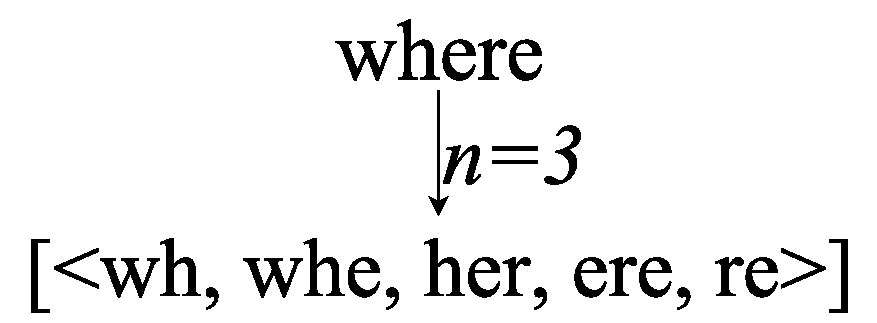
\includegraphics[max width=\linewidth,max height=8cm,keepaspectratio]{figures/fastText}
    \caption{An example of the n-grams derivation of FastText in~\cite{bojanowski2016enriching}}\label{fig:fastText}
\end{figure}

\subsubsection{The vocabulary issues}
\label{soaVocabulary}

Having good algorithms for word embeddings is a good starting point. But there may be some problems when deciding how to preprocess the corpora. What we want to consider as input features? Only the words in lowercase, cleaned up from all the non alphabetical characters, or we may consider other hints from the user typing such as capital letters or punctuation?

The choice is usually to clean deeply the inputs in order to reduce the vocabulary. For capitalization it means to lowercase everything. But the casing feature may be important in some way to help recognizing entities (think about a place name with capital letter, or an acronym uppercase). On the other side, beginning of sentences have capital letters that should be lowercased because that is not a wanted feature, it is only required by writing rules. For this reason some invented a truecasing model~\cite{lita2003truecasing} that aims at reconstructing the correct word casing.

The other critical point is punctuation: a decision is needed about whether to keep those signs as additional dictionary entries or simply drop them. A very critical one is the apostrophe: the words around it are usually modified, so not only they have to be considered separately, but also some reconstruction could be required (example: $``$\textit{we're}$"$  as a single word  \(  \left[ "we're" \right]  \)  or separating by the apostrophe  \(  \left[ "we", "'re" \right]  \)  or reconstructing the original words  \(  \left[ "we", "are" \right]  \)  in order to have the same entry for the verb  \( "are" \)  in the dictionary (or applying a stemmer with similar results).

An approach based only on alphabetical lowercased words may be good for scenarios where the users do not have the time to write complex punctuations. But when additional features are provided (such as punctuation and word casing in text, and accents and tone in voice), it would be a pity to throw away things that may be useful for doing a better classification.

\subsection{Intent classification}
\label{soaIntent}

Let us talk here about approaches for the first task of NLU, intent classification, that takes as input the sentence and provides as output a label that corresponds to the intent type of the sentence. It is a multi-class classification. It takes in input a sequence of words and produces a single label, that is a trait value of the input sentence.

\subsubsection{Keyword-based}
The first approach that can be considered is keyword-based. In this approach, for each intent type we determine a set of keywords that, if present in the current input, gives a score to the selected intent type. For example a naive classifier can be built to generate keyword groups from training sentences and classify accordingly to their presence by doing a $``$majority vote$"$  on the words of the current sentence.\footnote{\url{https://chatbotslife.com/text-classification-using-algorithms-e4d50dcba45}} This approach dynamically determines the keywords for each class, but it is not good enough because it looks only at some words in the current input sentence.

A better idea would be to compute a sentence-level representation that summarizes all the words and the meaning of the sentence, and from this vector it does a classification on the output labels (intent types). For this sentence vector a lot of different approaches can be applied that are explored in the following paragraphs.

\subsubsection{Average of word vectors}
First of all, given the word vectors for each word contained in the sentence, an average can be done. As shown in Figure~\ref{fig:intentAverage}, after the average is computed over the fixed-length embedding values for the input words, a simple feed-forward layer can be used to map to the intent space, producing logits that estimate the probability to belong to a certain class (intent type).

This strategy however is not good because it does not consider the order and the relationships between the words. The order matters a lot in natural language.

%%%%%%%%%%%%%%%%%%%% Figure/Image No: 11 starts here %%%%%%%%%%%%%%%%%%%%

\begin{figure}[!htbp]
    \centering
    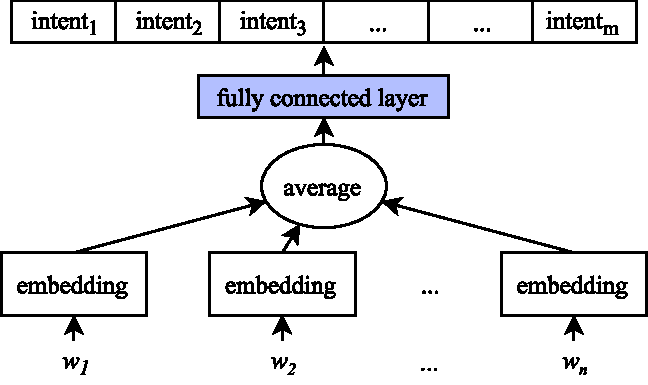
\includegraphics[max width=\linewidth,max height=8cm,keepaspectratio]{figures/intentAverage}
    \caption{Intent classification by average of word vectors}\label{fig:intentAverage}
\end{figure}

Another problem of this approach is that actually every word counts the same, so if stopwords are not eliminated they can bias the output basing on irrelevant inputs.

\subsubsection{RNN approach}
To consider the order, a RNN can be used to summarize the sentence and produce a sentence representation that can be used in another layer to classify on the intent types. The output of the RNN is taken only at the end of the sequence. This approach is able to capture some more information about the sequence that considers the relative order of words. Considering both a forward and a backward RNN, the output of the summarized output is not biased towards the end of the sentence as would happen for a forward-only RNN. Figure~\ref{fig:intentBidirectionalRNN} shows how the bidirectional encoding of the sentence substitutes the average operation with respect to the previous approach. The output projection layer finally performs the mapping to the intents spaces.

%%%%%%%%%%%%%%%%%%%% Figure/Image No: 12 starts here %%%%%%%%%%%%%%%%%%%%

\begin{figure}[!htbp]
    \centering
    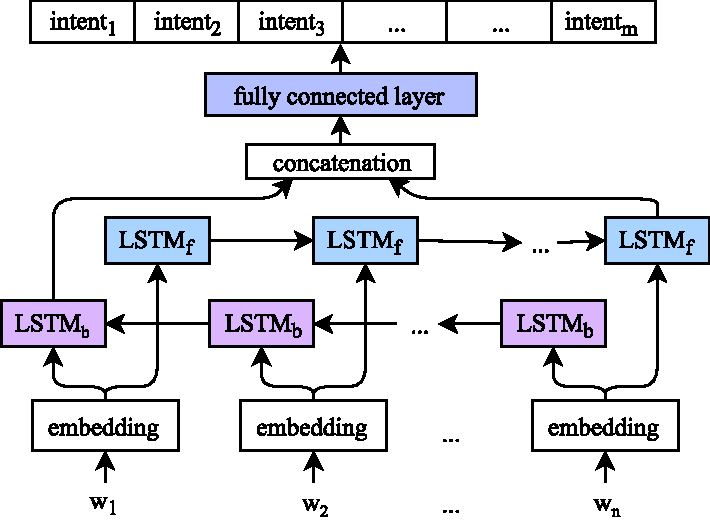
\includegraphics[max width=\linewidth,max height=8cm,keepaspectratio]{figures/intentBidirectionalRNN}
    \caption{Intent classification by applying a bidirectional RNN}\label{fig:intentBidirectionalRNN}
\end{figure}

What makes this technique to work well is that the LSTM is very good at capturing sequence-level information, considering with different importance the input words. The problem of stopwords is defeated and the Recurrent Network learns to discard the irrelevant words.

\subsubsection{RNN with attention}
To emphasize the fact that some words count more than others in the classification problem, several techniques can be used. First of all, \textit{stopwords} can be identified and removed. But more dynamic approaches can automatically learn a distribution over time of words that tells how much relevant is this word for the task. This is the attention mechanism, that is quite commonly adopted in automated translations~\cite{bahdanau2014neural} and on sentiment analysis~\cite{lin2017structured}.

This kind of additional component, as will be seen also for the slot filling task in \ref{sequenceAttention}, provides a way both to learn those scoring values and to use them for a weighted average on the outputs of the RNN layer. In the case of intent classification the attention wraps the bidirectional RNN.

\subsection{Sequence-to-sequence models for slot tagging}
\label{soaSeq2Seq}

The task of slot tagging instead consists of generating an output sequence in which each element corresponds to a tag for the corresponding input word. The tag can be the entity type or the IOB. IOB can be useful when there is the need to deal with multi-word slots, as in the example of Figure~\ref{fig:iob}.

A lot of the architectures listed below have been created for the task of Neural Machine Translation. This task takes as input the sequence of words in the source language and outputs a sequence of words in another language. This is somehow similar to the task of sequence labeling, because it maps an input sequence to an output sequence, but has some differences that make it a lot different and require a different approach. The differences will be explained in details during the analysis.

A common characteristic of them is the presence of two key elements: an encoder and a decoder. The encoder is responsible of collecting all the useful features on the input sequence. The decoder instead must generate the output sequence. The differences between the different models are on the way that the encoder provides input to the decoding stage. The general composition of such encoder-decoder approaches is shown in Figure~\ref{fig:encoderDecoder}

%%%%%%%%%%%%%%%%%%%% Figure/Image No: 13 starts here %%%%%%%%%%%%%%%%%%%%

\begin{figure}[!htbp]
    \centering
    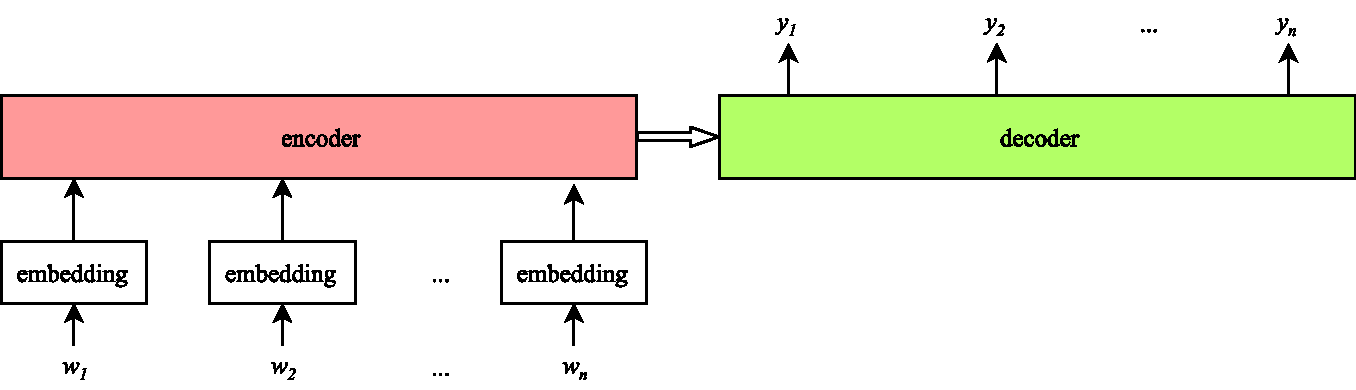
\includegraphics[max width=\linewidth,max height=8cm,keepaspectratio]{figures/encoderDecoder}
    \caption{The connections between Encoder and Decoder components for sequence translation}\label{fig:encoderDecoder}
\end{figure}

A very critical point when generating the output sequence is the correlation between the IOB labels. For example a $``$\textit{I-ent}$"$  is always preceded by a $``$\textit{B-ent}$"$  or another $``$\textit{I-ent}$"$ . Also there can be some patterns that highlight that after a certain entity it is more probable to find another one. This is called output dependency, that occurs at the decoding stage, just before the production of the outputs. 

Modeling the output dependencies can be done in different ways:

\begin{itemize}
	\item Local choice: using this approach, each decoding step produces an output that is then projected to the labels. The decision about which labels to assign is done locally, performing a simple softmax operation followed by a sampling;

	\item Feed the previous output together with the current input to decoding timesteps: (similarly to a Jordan Network~\cite{jordan1997serial}) in this approach, the output is fed back as input to the next timestep for the decoder network, and the network in training learns the output dependencies;

	\item Linear-chain CRF: an alternative to RNN for modeling the output dependencies is using a linear-chain CRF. This can substitute the decoder network, and use the encoder to produce its input features. CRF finds the paths with higher energy in a very similar way to RNN. In other words, it finds the output sequence that is mostly probable;

	\item Beam search: not only a single candidate is kept for subsequent decoding timesteps, but a set with fixed size, in order to be able to perform decoding without always following the local optimum.
\end{itemize}

In the following paragraphs we give a description of some sequence-to-sequence approaches, from the most simple ones towards the most suitable for the slot labelling task.

\subsubsection{Simple Encoder-Decoder}
The most simple approach, illustrated in figure~\ref{fig:encoderDecoderRNN} is the one where the encoder collects all the word vectors and using a RNN computes a final representation of the sentence (as in the intent classification task). This representation is passed to the decoder RNN that for each timestep produces an output word.

%%%%%%%%%%%%%%%%%%%% Figure/Image No: 14 starts here %%%%%%%%%%%%%%%%%%%%

\begin{figure}[!htbp]
    \centering
    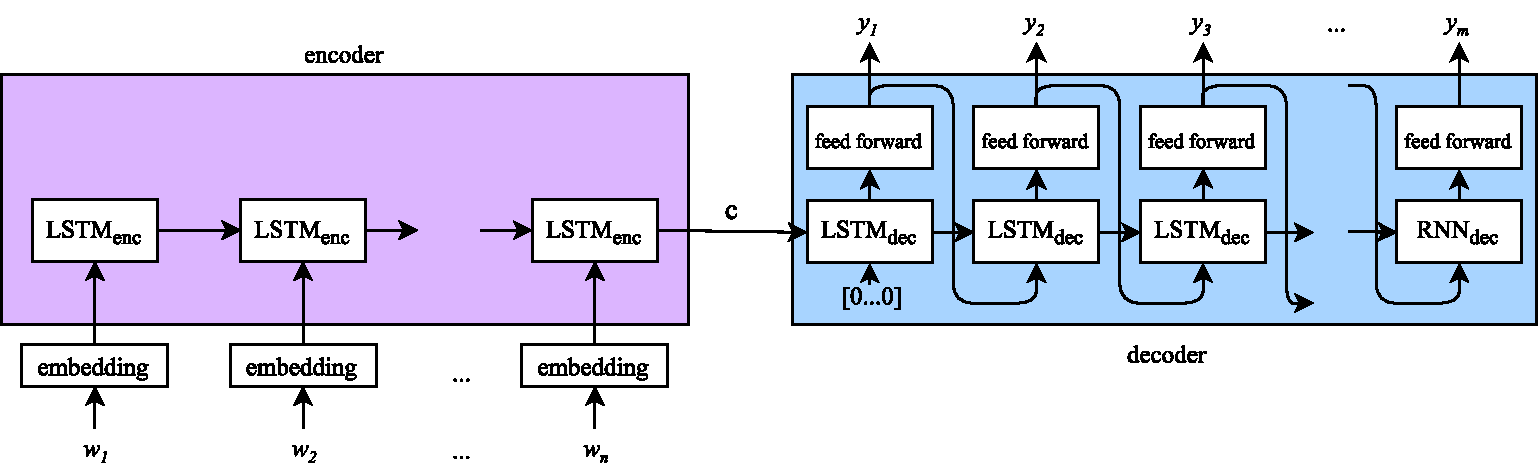
\includegraphics[max width=\linewidth,max height=8cm,keepaspectratio]{figures/encoderDecoderRNN}
    \caption{The usage of RNN for a simple Encoder-Decoder approach}\label{fig:encoderDecoderRNN}
\end{figure}

This model has some problems. First of all, the decoding part depends only on the sentence vector c, that must be able to keep all the information on the input sequence, whose length can vary, in a fixed size. Then, the decoding steps may easily lose the relevant information from this vector, since the decoding can take a lot of decoding timesteps. But a much greater problem comes from the lack of constraint on the output sequence length: in translation between different languages, this can be a good feature, but in our task of sequence labeling we want an output sequence with fixed length. The last observation we can make is that there is no alignment model between the input and output sequences. The outputs depend on all the inputs, without having different encoded information for the decoding of the output sequence.

\subsubsection{Encoder-decoder keeping sentence vector}
This model comes from~\cite{cho2014learning}, a study on the task of neural machine translation. It is an enhanced version of the previously considered model because the sentence vector coming from the encoding stage is passed to all the decoding stages (see Figure~\ref{fig:encoderDecoderKeepC}).

%%%%%%%%%%%%%%%%%%%% Figure/Image No: 15 starts here %%%%%%%%%%%%%%%%%%%%

\begin{figure}[!htbp]
    \centering
    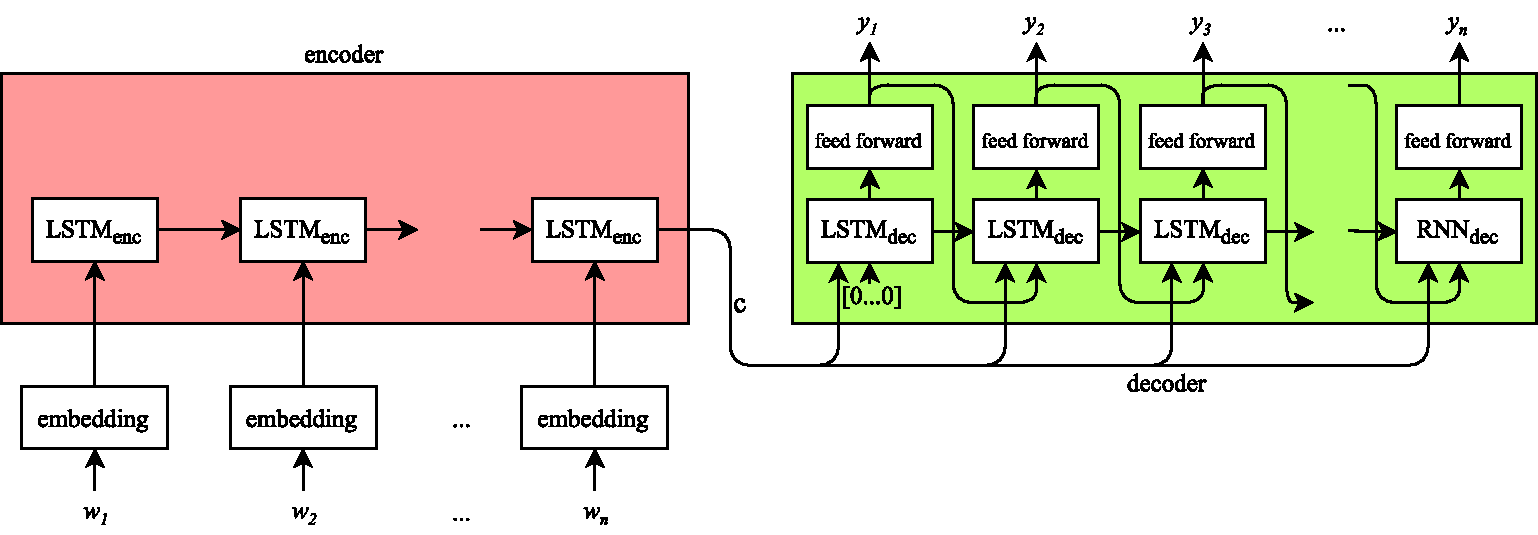
\includegraphics[max width=\linewidth,max height=8cm,keepaspectratio]{figures/encoderDecoderKeepC}
    \caption{Passing the sentence vector to all the decoding steps}\label{fig:encoderDecoderKeepC}
\end{figure}

This approach helps the decoding stages that, receiving the sentence vector directly, can perform better in their task. However, some problems are not solved: the output sequence length has no constraints and there is no alignment model.

\subsubsection{Encoder-decoder with aligned inputs}
This model was proposed~\cite{liu2016attention} for the sequence labeling problem (that can be applied to slot filling, POS tagging). In this model the encoder sends some information to the decoder for each input word instead of sending a single vector at the end (see figure~\ref{fig:encoderDecoderAligned}).

%%%%%%%%%%%%%%%%%%%% Figure/Image No: 16 starts here %%%%%%%%%%%%%%%%%%%%

\begin{figure}[!htbp]
    \centering
    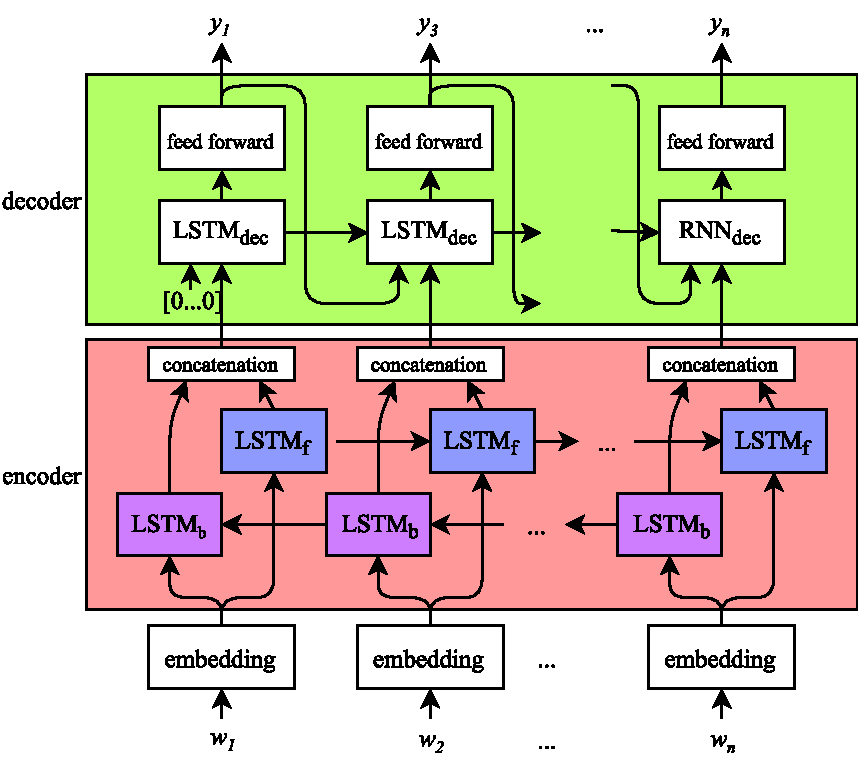
\includegraphics[max width=\linewidth,max height=8cm,keepaspectratio]{figures/encoderDecoderAligned}
    \caption{The Encoder-decoder with aligned inputs: each decoding step is influenced by the contextual representation of the aligned word}\label{fig:encoderDecoderAligned}
\end{figure}

This model fixes the output sequence length to the length of the input sequence. The alignment model is fixed: the decisions in decoding are done looking at current input word in the current left plus right context.

\subsubsection{Encoder-decoder with attention}
\label{sequenceAttention}

The idea of attention empowers recent studies on translation. The purpose is to decide which outputs of the encoder are more relevant for the current decoding step dynamically. On the previous model, always the aligned encoded input is used, but for language translation this can be a limitation.

Using the attention~\cite{bahdanau2014neural}, that provides a dynamic alignment model, it is possible to:

\begin{itemize}
	\item Determine which are the encoded inputs that are more relevant;

	\item Use them to provide a better translation.
\end{itemize}

%%%%%%%%%%%%%%%%%%%% Figure/Image No: 17 starts here %%%%%%%%%%%%%%%%%%%%

\begin{figure}[!htbp]
    \centering
    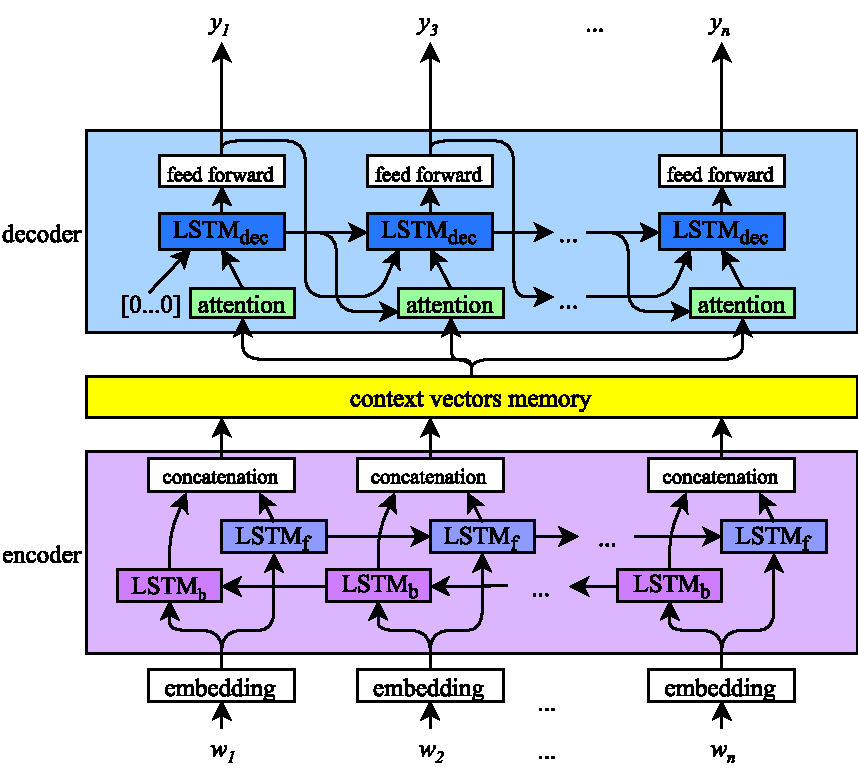
\includegraphics[max width=\linewidth,max height=8cm,keepaspectratio]{figures/encoderDecoderAttention}
    \caption{The aligned Encoder-decoder with the addition of attention mechanism}\label{fig:encoderDecoderAttention}
\end{figure}

The attention, as can be seen in Figure~\ref{fig:encoderDecoderAttention}, adds two blocks: one is the context vector memory, which stores the output of the bidirectional RNN at each timestep, and the other one is the attention block that is responsible to pick up the correct mix of the encoded vectors by doing a weighted sum of them and provide that to the decoder RNN. 

By looking inside at the \textit{attention} mechanism, in Figure~\ref{fig:attention} we can see that the encoded vectors  \( e \)  are used together with the previous hidden state of the decoder cell  \( h_{i-1} \) in some matricial multiplications and finally pass through a softmax. This part is responsible to learn the weights for each timestep of the decoder that represents how much relevant are the input words for the determination of the current output word. The matrices  \( W_{1} \) , \( W_{2} \)  and  \( V \) are used together with a  \( tanh \)  layer to determine dynamically those weights. This block, put inside a complex network architecture, learns all the parameters thanks to the backpropagation algorithm being end-to-end differentiable. The output  \( c_{i} \)  is then computed doing a weighted sum between the  \( e_{j} \)  encoded vectors.

%%%%%%%%%%%%%%%%%%%% Figure/Image No: 18 starts here %%%%%%%%%%%%%%%%%%%%

\begin{figure}[!htbp]
    \centering
    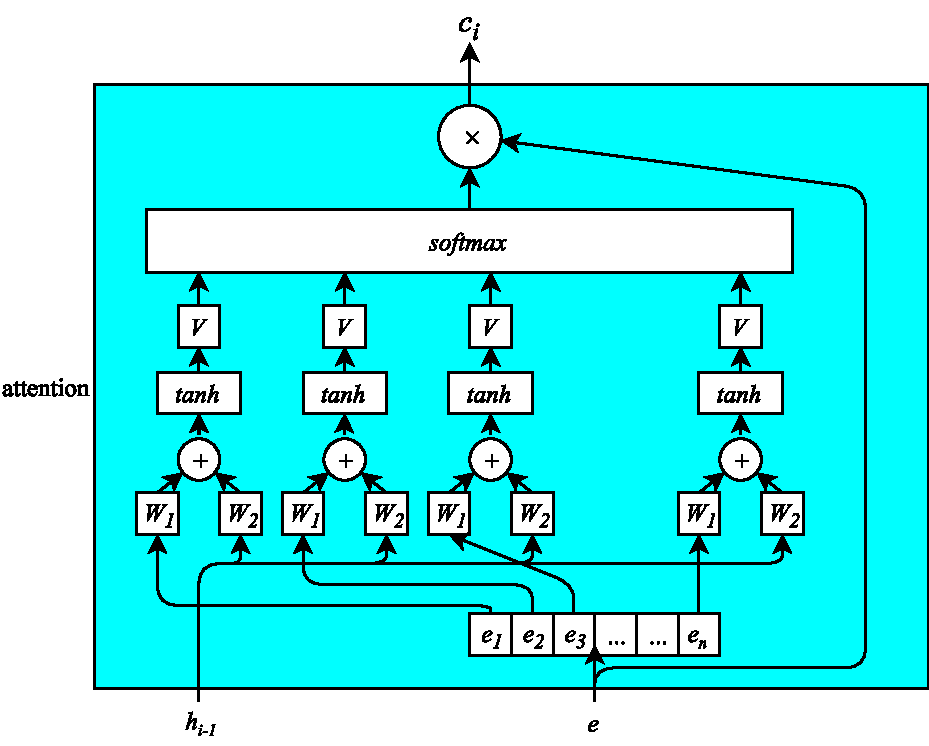
\includegraphics[max width=\linewidth,max height=8cm,keepaspectratio]{figures/attention}
    \caption{How the Attention block computes a weighted sum, learning the weights dynamically}\label{fig:attention}
\end{figure}

With this network, used for translations, it is useful to show how the attention maps the words in the two languages. Figure~\ref{fig:attentionVisualization} shows a matrix representation that says which input words were used to provide the corresponding output words.

%%%%%%%%%%%%%%%%%%%% Figure/Image No: 19 starts here %%%%%%%%%%%%%%%%%%%%

\begin{figure}[!htbp]
    \centering
    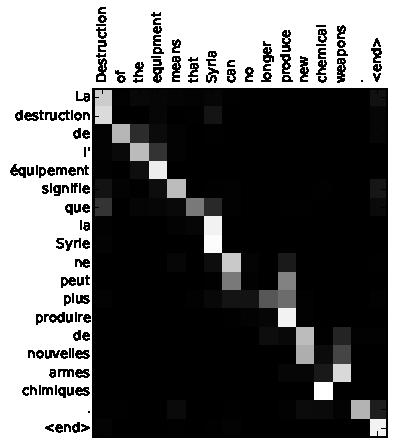
\includegraphics[max width=\linewidth,max height=8cm,keepaspectratio]{figures/attentionVisualization}
    \caption{A visualization of the attention scores in translation~\cite{bahdanau2014neural}}\label{fig:attentionVisualization}
\end{figure}

The attention model is quite advanced, and since a lot of other parameters are there in the network, a lot more of training samples must be used.

For the task of sequence tagging it seems to be too much. The output labels depend only on the current word context that is already given by the bidirectional encoder RNN, so the expected values for the attention distribution is that it will keep the inputs and outputs aligned. It can be kept together with the aligned model just to provide more features.

\subsection{Joint tasks}
The two tasks can be combined together in one single network in different ways and with a wide variety of additional things that can be added (for example attention mechanism, output dependencies). The approaches found in literature try to use a common encoding stage and then differentiate on the decoding, one for each task. The network has to fork at some point because the shape of the outputs is different: one single label for the intent and many slot labels, considering a single input sentence.

In~\cite{liu2016attention} there are two different proposed architectures: one is based on the encoder-decoder adding the intent output, while the other collapses all in one single compact structure.

The first one, as can be seen in Figure~\ref{fig:jointSLUAligned}, is a combination of the bidirectional RNN for intent classification and the encoder-decoder with attention for the slot filling. The two networks, having the encoder in common, are merged together, and fork for the following layers towards two different outputs.

%%%%%%%%%%%%%%%%%%%% Figure/Image No: 20 starts here %%%%%%%%%%%%%%%%%%%%

\begin{figure}[!htbp]
    \centering
    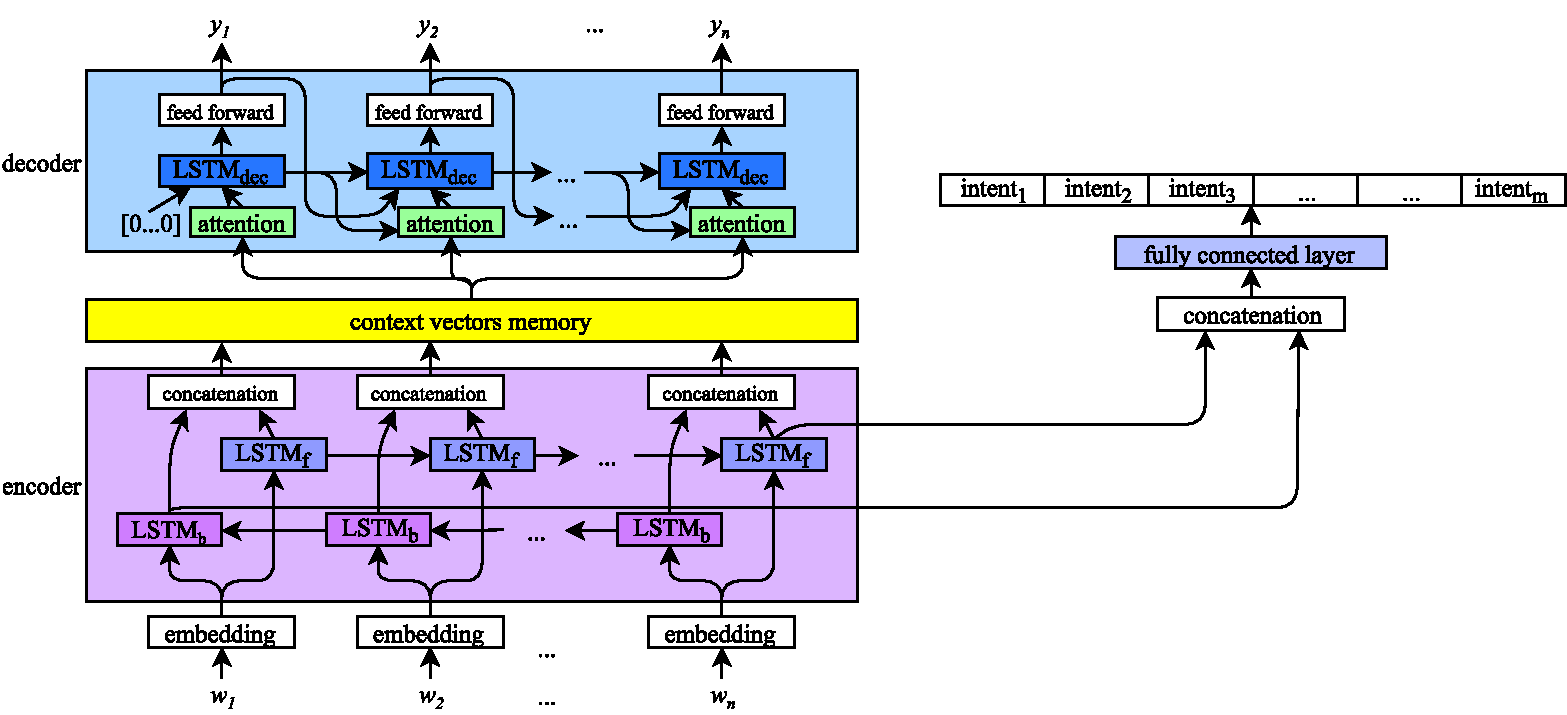
\includegraphics[max width=\linewidth,max height=8cm,keepaspectratio]{figures/jointSLUAligned}
    \caption{The Joint Encoder-decoder model with Aligned Inputs in~\cite{liu2016attention}}\label{fig:jointSLUAligned}
\end{figure} 

The two branches consider different outputs of the encoder. The intent classifier is added as a branch that takes the last state of the encoder and then projects to the intent space with a single layer feedforward. Instead the slot filling decoder takes all the word-level outputs because it needs an aligned model.

The other network proposed in the paper is a bit different. Instead of having a separate RNN for encoder and decoder, it has a single bidirectional RNN, that in the forward direction also has the modeling of slot label dependencies. As can be seen in Figure~\ref{fig:jointSLUrnn}, the intent classification is done on top of the bidirectional RNN output, doing a mean pooling on the states at each timestep or, if the attention is enabled, by using a weighted average.

%%%%%%%%%%%%%%%%%%%% Figure/Image No: 21 starts here %%%%%%%%%%%%%%%%%%%%

\begin{figure}[!htbp]
    \centering
    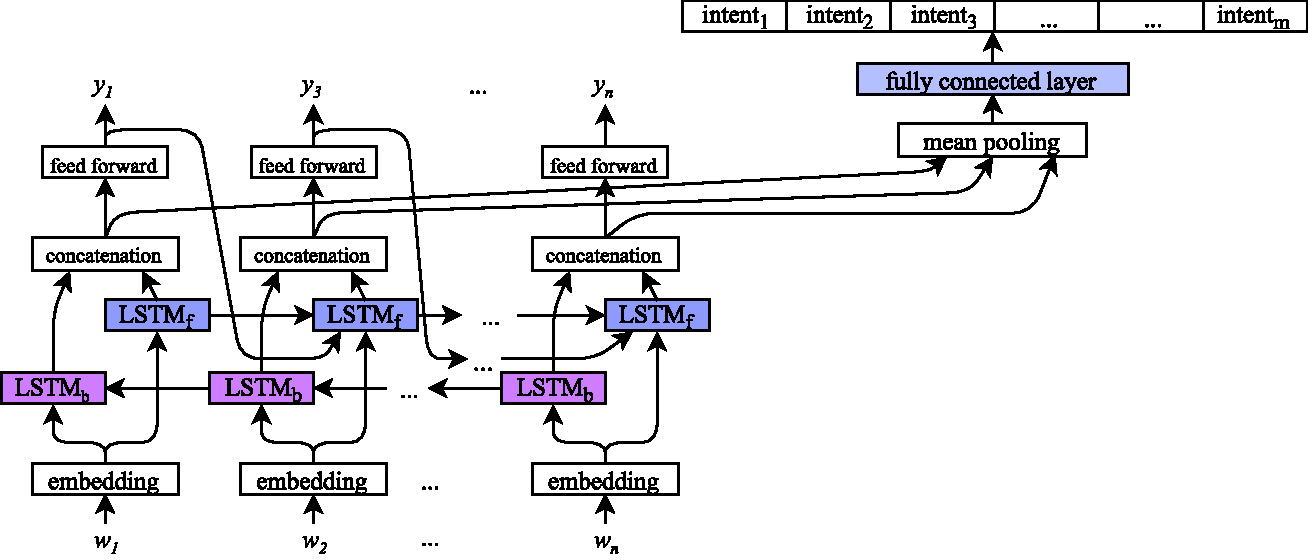
\includegraphics[max width=\linewidth,max height=8cm,keepaspectratio]{figures/jointSLUrnn}
    \caption{The joint attention-based RNN Model in~\cite{liu2016attention}}\label{fig:jointSLUrnn}
\end{figure}

\subsection{The interaction context}
\label{soaInteractionContext}

All the previously described networks only care about the current sentence, but human natural language understanding does not limit itself on this strict form. What happens when we meet some people that are already talking about something? It may take some time to understand the topic of the discussion, we need to collect some information as the interaction goes on to get the point of the discussion. This happens because most of the sentences are not standalone, but they belong to a context that goes beyond the single sentence.

The \textit{context} of a conversation can be defined as a set of important things to know in order to both understand others and say more relevant things. The context can capture features belonging to different areas:

\begin{itemize}
	\item domain: knowledge of the topic of the discussion. A conversation where the participant have a deep knowledge of it brings an exchange of meaningful ideas and opinions;

	\item interaction: going beyond the fixed form of atomic question-answer pairs. Human to human conversations rely a lot on the interaction context, referring explicitly or implicitly to things that have been previously said. A multi-turn environment can allow users to do questions and later refining them to find what they were searching for, by simply adding new parameters instead of rebuilding a complete independent interrogation, or doing follow-up questions on the previous results;

	\item interlocutor: knowing better the user that we are interacting can be advantageous to find better and targeted responses to his question, both in the form and in the content.
\end{itemize}

In this work we focus more on the interaction context because it is the one that is mostly related to language. The domain knowledge is instead given by design in goal-oriented bots, because they are built to serve some specific needs and do restrict the topics of conversation. Instead for the interlocutor/user context, it is the field where the personalization techniques are analyzed, as will be seen in Section \ref{soaPersonalization} for the background and in Section \ref{approachPersonalization} for more dialogue-related personalization techniques.

The interaction context feature can be seen as some kind of memory that actors in a conversation need to keep about previous sentences. The context is necessary to understand the dialogue at different levels:

\begin{itemize}
	\item Understand the role of some words in a sentence given some information contained in other sentences. This practically means to identify entities by knowing that after a certain type of question it is easier to find them (e.g. replying to $``$\textit{Where?}$"$  questions suggest that the next sentence contains a place entity, even if the sentence does not contain indicators like $``$\textit{near/in/at}$"$ ). We may call this setting \textit{multi-turn slot filling}.

	\item Understand the meaning of the current sentence. This is the case of sentence classification, like extracting the intent, when the current sentence does not give hints about it, but a knowledge of the previous sentences can lead to the correct understanding (e.g. replies like $``$\textit{ok. Let's do it}$"$  that standalone are impossible to be processed). We call this the \textit{multi-turn intent classification}.

	\item Ability to link the all the entities that are mentioned in a discourse, being able to resolve the things that are behind words like $``$\textit{this/him}$"$ . This is the \textit{coreference resolution}.

	\item Based\ on previous levels, link the meanings of things across the different turns, and be able to answer to some test questions that require reasoning. This is the so called  \textit{dialogue tracking}.
\end{itemize}

All those levels of understanding provide active fields of research in the NLP community and they fall under different names. The first one is \textit{multi-turn} appearing in~\cite{chen2016end},~\cite{chen2017dynamic},~\cite{xu2014contextual},~\cite{bhargava2013easy} and~\cite{shi2015contextual}. This term is specific to virtual assistants and it covers the first two levels of understanding: the goal is to identify the intent and entities in a dialogue where the user is not using a single sentence to ask for information. One common case is when, after the initial question of the user, the agent asks back for some clarifications or missing parameters to refine the search. In this case the assistant should put together the information contained both in the current sentence and in the previous ones, to perform a complete query. Other common cases are user follow-up questions. Receiving some results from the agent, the user could ask for more details or to change some parameters. In this case, the user refers to the previous query and it is only changing some constraints (like the intent or some slots).

The other used term is \textit{dialogue state tracking}: mostly known because of the Dialogue State Tracking Challenge~\cite{williams2013dialog}, it refers to the ultimate level of understanding a dialogue: represent the dialogue state and updating it as the conversation keeps going on.

Different solutions exist and depend on where we want the neural network to come in contact with the application logic (what to establish as manual rules and what is inferred by the neural network approach). Literature shows case studies where there is a strict separation between the understanding module and the management of the dialog state~\cite{liu2016attention}~\cite{chen2016end}, but also cases where everything is put together in an end-to-end fashion in a way more independent from domain rules~\cite{serban2016building}~\cite{eric2017key}.

In the first type of systems, the NLU module contains the recurrent neural network stuff and produces as output intent and slots. Once they are extracted from the dialogue, another module $``$dialogue state tracker$"$  keeps track of the conversation and applying some handwritten rules decides the flow of the conversation and provides responses back to the user.

Instead in the end-to-end architectures, all the components are trained by dialog examples. The positive point is that there is no need to handwritten rules for the dialogue state tracker. The rules are inferred by the dialog corpus and the system learns what is the most appropriate answer to provide. Some parts are still not part of the trainable model: the module accessing the data exposes some operations via some API. The trainable model learns when to issue API calls. However, the end-to-end approaches need a very big amount of dialogues to induce the general rules giving an advantage to rule-based dialogue tracking systems where the resources are limited.

The following paragraphs explore the three levels of interaction context that have been outlined previously.

\subsubsection{Multi-turn Understanding}
As mentioned before, the goal of multi-turn SLU is simply to extract the intent and the entities when the user is not providing a single sentence with all the required parameters. In a second moment, it could be after the agent asks back for some parameters, other sentences complete the initial one with more entities that are used to refine the search. It can be seen as an iterative filling of a fixed-structure form. For this reason, a naive approach could be simply to classify the intent on the first sentence and then collecting the parameters in a key-value fashion (the key is the name of the slot, that is asked by the agent, and the value is the answer taken $``$as is$"$ , as can be seen in Figure~\ref{fig:multiTurnFilling}).

%%%%%%%%%%%%%%%%%%%% Figure/Image No: 22 starts here %%%%%%%%%%%%%%%%%%%%

\begin{figure}[!htbp]
    \centering
    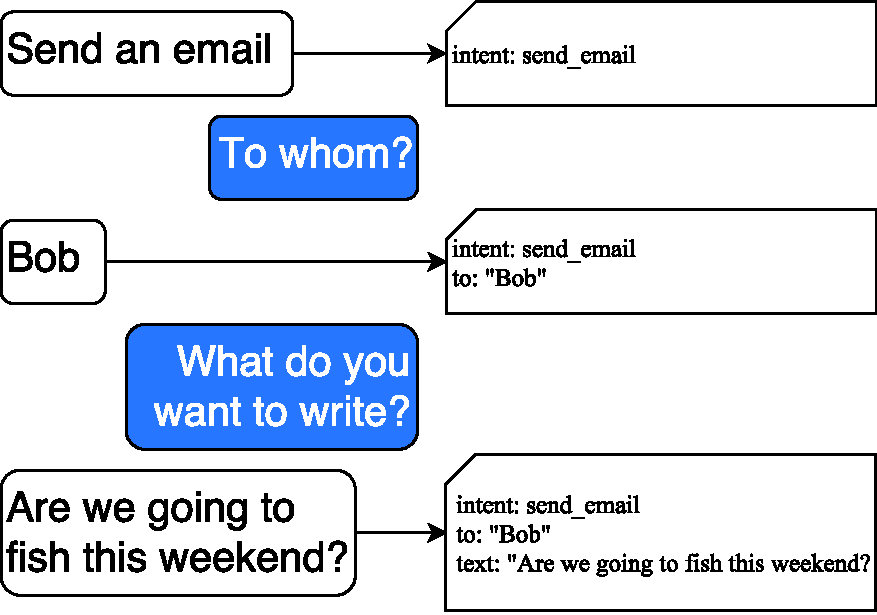
\includegraphics[max width=\linewidth,max height=8cm,keepaspectratio]{figures/multiTurnFilling}
    \caption{A simple dialogue where a simple key-value approach can provide multi-turn abilities}\label{fig:multiTurnFilling}
\end{figure}

This approach is quite simple but has some problems: this is not natural language. Natural language dialogue has not this fixed structure, and the system must be able to receive a sentence that contains more than a single entity. Another issue is that the user may change his mind in the middle of the interaction and start a new intent. For those reasons the SLU task should be expanded to the multi-turn environment by a more complete approach. We will there analyze some proposed solutions to this problem.

Some first works in the direction of contextualized understanding have been done in~\cite{xu2014contextual} for classification of the domain (that can be seen as a coarse-grained intent). In that work, the previous output of the system is added to the inputs by enlarging the input word vectors. The authors choose as approach for single-turn developed using a  CNN~\cite{krizhevsky2012imagenet}, so the multi-turn adding the recurrent connections results in a RNN/CNN hybrid network.

Another approach that has been studied for the multi-turn problem is~\cite{chen2016end}. The idea to additionally incorporate contextual knowledge is applied with a sentence encoder that considers also previous sentences. The current sentence is processed by a RNN like in~\cite{liu2016attention}, and the addition is the contextual sentence encoder that can be seen in Figure~\ref{fig:contextualSLUchen}.

%%%%%%%%%%%%%%%%%%%% Figure/Image No: 23 starts here %%%%%%%%%%%%%%%%%%%%

\begin{figure}[!htbp]
    \centering
    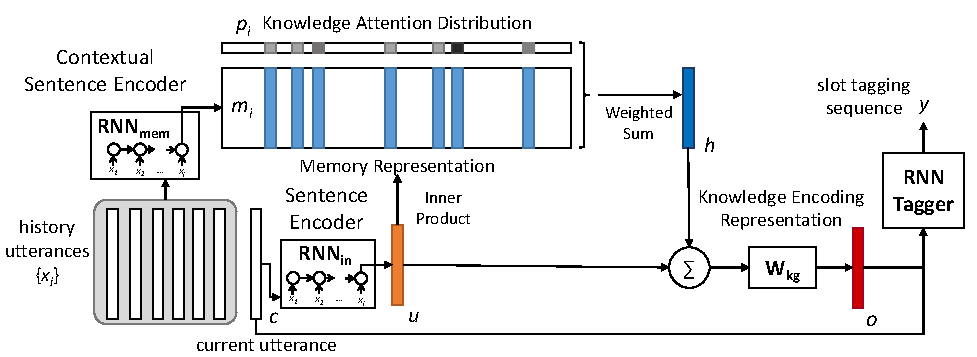
\includegraphics[max width=\linewidth,max height=8cm,keepaspectratio]{figures/contextualSLUchen}
    \caption{The contextual approach based on memory of previous turns in~\cite{chen2016end}}\label{fig:contextualSLUchen}
\end{figure}

This encoder provides a context memory representation, where each previous turn is represented. To choose which turns are more relevant for the current sentence, an attention mechanism is used in the encoded representation space. Weights for attention are computed by an inner product between the current sentence and the memory representations, which represent a measure of similarity of the considered pairs. The hypothesis behind this scoring is that sentences that have similar encoded representation should be considered more than the ones that are different. The final output of the encoding procedure is computed as the sum of the current sentence and the weighted sum of memory representations. During the decoding stage, similar to the one in~\cite{cho2014learning}, the encoded representation is used to generate slot labels.

The results of this approach have been evaluated on a proprietary dataset and therefore the results cannot be compared with other studies on the field. Furthermore in the paper the intent network is not described at all. However, this study is interesting in the perspective of how the previous sentences are considered together with the current one for the slot-tagging task.

A problem of this architecture is that the agent sentences are not considered. But the agent sentences could contain some keywords that may help to identify the slot in the decoding stage. For example if a trip requires a source and a destination, the agent asked for the source and the user answered with that, it is very relevant for the task of slot filling to know that the agent asked for source and not for the destination.

Another work has been done in~\cite{chen2017dynamic} on the value of time and roles in conversation. About the time, the idea is that most recent sentences count more and an attention score is given with values that fade out as the time is more remote. Instead for the roles, two similar networks are used, one for each role.

%%%%%%%%%%%%%%%%%%%% Figure/Image No: 24 starts here %%%%%%%%%%%%%%%%%%%%

\begin{figure}[!htbp]
    \centering
    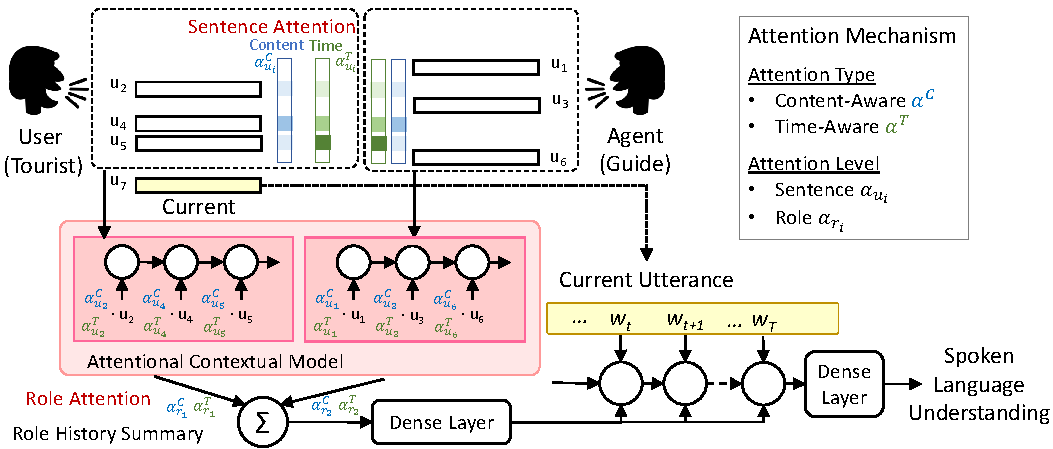
\includegraphics[max width=\linewidth,max height=8cm,keepaspectratio]{figures/timeRoleSLUchen}
    \caption{The time and role aware approach of~\cite{chen2017dynamic}}\label{fig:timeRoleSLUchen}
\end{figure}

We can see from Figure~\ref{fig:timeRoleSLUchen} that the history of sentences is encoded with different networks, one for the tourist and one for the agent. Two different mechanisms of attention are used: one is the content-aware, that is computed in the same way as in the previous mentioned paper with a dot product in the embedding space; the second one is the time-aware, that gives higher importance to recent sentences.

In this case the work has been done on the DSTC4 dataset\footnote{\url{http://www.colips.org/workshop/dstc4/}} that contains human-to-human dialogues. One of them is a tourist and the other one is a guide.

It can be seen with the progress of the DSTC over the years, that the task is switching from a multi-turn understanding to an end-to-end goal-oriented dialogue learning, as will be seen in the last paragraph of this subsection focused on DSTC6.\footnote{\url{http://workshop.colips.org/dstc6/}}

\subsubsection{Coreference resolution}
\label{soaCoreference}

The problem of coreference resolution is one of the most difficult to solve in NLP. There are currently models available to resolve explicit coreferences, using some correlation of gender and number between the entities and further references.

The problem of coreference resolution has been analyzed in TREC10,\footnote{\url{https://trec.nist.gov/pubs/trec10/t10\_proceedings.html}} as the main purpose of using the context in the sentences. In~\cite{harabagiu2001answering} a set of elements in the question, that may indicate entities mentioned in previous questions and answers, are searched. Those can be split into explicit references (such as pronouns like $``$\textit{this/that/him}$"$ , use of definite nominals like $``$\textit{the state}$"$  that suggest having a previous knowledge of reference) or implicit ones (like ellipsis of something that logically needs to be kept into consideration). The proposed system tries to find in previous turns the ones that contain the referenced entity.

A more complex approach has been analyzed by~\cite{sun2007discourse}, based on the Centering Theory~\cite{grosz1995centering} that models the local coherence of a discourse and how the transitions caused by a new sentence changes the center of the talk. In this work, two types of context are found: one depending on the user (analyzed by later TREC contextual tracks, corresponding to personalization techniques that will be analyzed in section \ref{soaPersonalization}) and the one of the discourse. The question processing should, according to the authors, perform three main tasks: \textit{(1)} question type analysis and categorization, \textit{(2)} detailed processing to build and expand queries, \textit{(3)} anaphora resolution. This theory is used to build a model that selectively retain query terms from previous interactions.

Going on more recent approaches to the coreference resolution problem,~\cite{de2015modeling}\ builds a model  for predicting the lifespan of discourse entities, in other words if one of them is a singleton entity or is referenced many times. The actual scores make clear that this is yet an open field of research, where only simple sentences achieve great accuracy. A detailed description of this model is explained in an interesting online article\footnote{\url{https://medium.com/huggingface/state-of-the-art-neural-coreference-resolution-for-chatbots-3302365dcf30}} and available as an online demo.\footnote{\url{https://huggingface.co/coref/}}

\subsubsection{Simple QA to test the memory}
Going beyond the quite simple tasks of entity recognition and coreference resolution, some more difficult challenges try to address the question-answering (QA) problem relatively to the discourse. The idea is to provide some sentences that contain factual information and then an easy question is asked about this. The system has to use correctly memory abilities and combine the different facts to provide the response.

On the easiest problems proposed in~\cite{weston2015towards}, the information is contained in simple sentences that are composed by triples of subject, verb and object. Usually a model of memory~\cite{sukhbaatar2015end} is used to store the relationships between the entities expressed by the triples. From this memory the easiest questions can be directly provided, while for tasks like counting on temporal reasoning it is necessary to enable a process of machine reasoning to turn the facts into operational knowledge. Some examples can be seen in Figure~\ref{fig:toyQuestionsMemory}.

%%%%%%%%%%%%%%%%%%%% Figure/Image No: 25 starts here %%%%%%%%%%%%%%%%%%%%

\begin{figure}[!htbp]
    \centering
    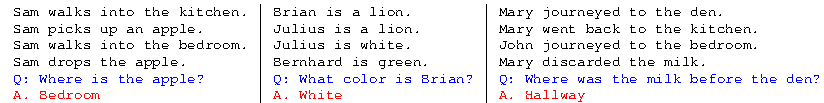
\includegraphics[max width=\linewidth,max height=8cm,keepaspectratio]{figures/toyQuestionsMemory}
    \caption{An example of the questions asked in~\cite{weston2015towards}}\label{fig:toyQuestionsMemory}
\end{figure}

The memory model can be seen as a $``$soft$"$  hash table. It stores key-values pairs. The output of a lookup is a weighted sum of the values, where the weights are attention weights derived by the training procedure.

\subsubsection{End to End for Goal-oriented dialogues}
More specifically to the interaction context for goal-oriented dialogues, the DSTC6,\footnote{\url{http://workshop.colips.org/dstc6/}} rebranded as \textit{Dialog System Technology Challenges}, has a dedicated track for this objective\footnote{\url{http://workshop.colips.org/dstc6/papers/track1\_overview\_perez.pdf}} and is composed of the following tasks:

\begin{itemize}
	\item Issuing API calls: asking to the user the required parameters until a complete interrogation is performed;

	\item Updating API calls: the user asks to modify an existing request;

	\item Displaying options: when multiple results are found, the bot should provide a list of the most relevant and manage the user choice between them;

	\item Providing extra information: after that a result has been chosen, the user can ask for extra information about the corresponding entity.
\end{itemize}

What is special of this challenge is the end to end trainability of the systems involved. The Natural Language, that is very flexible and various, is put in contact with APIs that instead are very fixed and must follow strict rules. Having an end-to-end differentiable system allows to use the approaches on new problems and domains by simply having a huge corresponding training corpus. Removing the domain-specific handcrafting provides more versatile systems that can fastly be used for new domains.

The origins of these approaches come from the generative chit-chat dialogs. From corpora of discussions (forum threads / movie conversations), the system is trained in a end-to-end fashion to predict the next sentence. The porting from this scenario to goal-oriented ones has some issues that generate from the fact that the conversation is intrinsically different in the purpose: the system is interrogated by the user and has to provide some information back. Beyond keeping the conversation smooth, the agent has to ask questions to the user to have a better formulation of the request, query knowledge bases, interpreting the results and provide them to the user in the correct shape in order to complete a transaction.

For these reasons, in this type of system, the outputs are both the agent responses and the API calls. Not only the understanding part is turned from handcrafted rules to an optimization problem, but also the replying part. The API to call are determined without using fixed rules, but with a model that is determined by the training corpus. The same applies to the response generation: there are not fixed rules deciding what to say in responses.

A critical challenge for generative systems is to keep the coherence between turns and be more focused on the topic of the dialogue, discarding irrelevant responses that do not provide the required information. This problem is addressed by two different things: one is having the training corpus focused on the selected domain, and the second one is to maintain the topic by using some models like in~\cite{xing2017topic} that biases the output sentences by giving more topic attention.

A point that still needs handcrafted features is the KB interrogation through fixed APIs. One of the reasons that drives this choice is that a legacy system may be used as KB and it can have a predefined set of operations that cannot be modified. Another reason could be that those APIs belong to third parties, like web services, that have strict calling rules. However some works have been done also towards a more dynamic exploration of information like discussed also in the classification done in \ref{soaClassificationApproaches}.

For example at Stanford they experimented with a data exploration that can be explored as a set of key-value pairs. In this way the system, trained in an end-to-end fashion will be able to explore the KB in a more dynamic and content-aware way with structured data~\cite{eric2017key}. It learns how to extract information from a KB without the need of handcrafted dialogue state tracking. This is possible thanks to the KB structure that enables a good exchange of data between the conversation and the KB without the need of intent tracker and relying only on latent neural embeddings. This approach is mainly a sequence-to-sequence generator enriched by a KB that provides triples of \textit{subject, relation, value}. The values are available to the output generation thanks to some placeholders in the output dictionary in the form of \textit{subject\_relation}, that is later replaced by its value after decoding.

As can be seen, all those approaches really combine the techniques of generative conversations together with goal-oriented interactions.

\subsection{NLU as a service}
As of today, there are a lot of platforms that provide Natural Language Understanding in the form of Software as a Service (SaaS). Big companies have decided to invest on it, to be the ones that hold the technology. They made those topics extremely easy for the developers who via a web interface can create dialogue flows and annotate manually the data. There is no need to know about the technology that is inside. All it is needed for a developer is to understand the jargon used by the platform and configure a black box.

%%%%%%%%%%%%%%%%%%%% Table No: 2 starts here %%%%%%%%%%%%%%%%%%%%

% !TEX encoding = utf8
% !TEX root = ../main.tex

\begin{table}
  \begin{tabularx}{\textwidth}{rcccccccX}
    \toprule
    \textbf{Provider}&
    \textbf{Deployment} &
    \textbf{\begin{turn}{90}Messenger platforms integration\end{turn}} &
    \textbf{\begin{turn}{90}intent\end{turn}} &
    \textbf{\begin{turn}{90}slots\end{turn}} &
    \textbf{\begin{turn}{90}required parameters management\end{turn}} &
    \textbf{\begin{turn}{90}end-to-end trainable\end{turn}} &
    \textbf{\begin{turn}{90}pre-defined intents\end{turn}} &
    \textbf{\begin{turn}{90}open source\end{turn}} \\
    \midrule
    wit.ai & web service & \ding{55} & \ding{51} & \ding{51} & \ding{55} & \ding{55} & \ding{55} & proprietary \\
    DialogFlow & web service & \ding{51} & \ding{51} & \ding{51} & \ding{51} & \ding{55} & \ding{51} & proprietary \\
    LUIS & web service & \ding{51} & \ding{51} & \ding{51} & \ding{55} & \ding{55} & \ding{55} & proprietary \\
    IBM & web service & \ding{55} & \ding{51} & \ding{51} & \ding{51} & \ding{55} & \ding{55} & proprietary \\
    alexa & web service & \ding{51} & \ding{51} & \ding{51} & \ding{51} & \ding{55} & \ding{51} & proprietary \\
    recast.ai & web service & \ding{51} & \ding{51} & \ding{51} & \ding{55} & \ding{55} & \ding{51} & partially open \\
    RASA & self & \ding{51} & \ding{51} & \ding{51} & \ding{55} & \ding{51} & \ding{55} & open \\
    \bottomrule
  \end{tabularx}
  \caption{A comparison between the major NLU providers}\label{tab:soaNLUproviders}
\end{table}


Those platforms usually provide intent classification and slot filling, with an approach that is not usually trainable in a end-to-end way. The provided features, as can be seen in Table~\ref{tab:soaNLUproviders}, turn the user sentences in structured data. Some platforms offer a way to force the user to provide some parameters (compulsory entities for some intents), managing the questions that the bot should ask when they are missing and call the fulfillment endpoint (the service owned by the developers of the bot, receiving the structured data) only when those parameters have been provided. The programmers are left to the role of handling the dialogue state, retrieving the information and providing a response.

But this does not scale well when the dialogue can have lots of different states and the user could change the topic of conversation in every moment. In those situations, the task of handcrafting rules to track the state of the conversation can become quite difficult. Also when something in the behaviour of the bot is not correct, the investigation of the problem can be cumbersome. Instead if the dialogue-state-tracking and the dialogue itself are trained end-to-end, changing the behaviour is as easy as adding a new example to the training corpus.

This kind of end-to-end trainability is supported on the shelf by RASA,\footnote{\url{http://rasa.com/}} an open source tool that has two main components: the NLU and the dialogue management Core. The first one turns sentences into intents and entities, while the second one manages the state of the conversation and determines responses and API calls without handcrafted rules. The developers of a bot using this libraries have to define the intents, entities, the actions (that correspond to some methods) and templates (for the responses) and provide examples for training both the NLU and the core.

There have been some efforts to compare the performances of all those systems by SNIPS,\footnote{\url{https://snips.ai/}} that tested a lot of those platforms to compare the results mainly on the intent detection task. The benchmark does also compare the results on out-of-domain samples, that are sentences that should be classified with none of the declared intents and managed with fallback options. The results are available both on their site,\footnote{\url{https://snips.ai/content/sdk-benchmark-visualisation/}}\footnote{\url{https://www.slideshare.net/KonstantinSavenkov/nlu-intent-detection-benchmark-by-intento-august-2017}} and most importantly the datasets used are available with an open license.\footnote{\url{https://github.com/snipsco/nlu-benchmark}}

 %%%%%%%%%%%%  Starting New Page here %%%%%%%%%%%%%%

\section{Personalization}
\label{soaPersonalization}

This section analyzes the state of the art of personalization, starting from how to profile users and determine their features in \ref{soaPersonalizationFeatures}, and considering the existing approaches for recommender systems and their problems in \ref{soaPersonalizationRec}. Finally, we discuss the so-called cold-start problem, particularly relevant in a conversational agent interaction scenario..

We use the following definitions for personalization and recommendation:

\begin{itemize}
	\item Personalization: a general technique to change the behaviour of a system depending on the user with the intent to lead better experience;

	\item Recommendation: a technique whose goal is to provide content that may be interesting according to user history, item catalogue and business objectives.
\end{itemize}

\subsection{User features and Personality analysis}
\label{soaPersonalizationFeatures}

A personalization or a recommender system need in input some information about the user in order to provide some outputs. Those information can be provided explicitly by the user, for example by asking him to fill up a questionnaire, or can be collected implicitly, analyzing his behaviour and doing some forecasts.

While having those features provided directly by the user is straightforward to be done, the implicit discovery is a bit more challenging. However users may not want to tell their personal details to the system to receive targeted recommendations. It is something that is not seen as good, because personal details are sensible data and no one wants to share them. Also when receiving explicit self-judgement from users, a big problem is how to trust them. For those reasons the implicit discovery of some features may help in different ways: looking at some available data and behaviour of the user personal details can be estimated and users can be clustered together considering some dimensions that may reflect sensible data and their personality.

With the spread of social networks a lot of data is ready to be analyzed to build big models that are able to predict personal information. The most common nowadays, Facebook, stores information of any kind about users: from age, occupation, and other personal information to others relative to interests. This is the ideal setting for training models that predict some user features based on others, contained themselves on the social network or coming from other sources. Specially on the fields of social sciences and personality analysis~\cite{kosinski2015facebook}.

For example, one of the biggest datasets to perform personality analysis is the myPersonality dataset.\footnote{\url{https://www.psychometrics.cam.ac.uk/productsservices/mypersonality}} Born as an application to take psychometrics tests and allowing users to give access to their personal data on Facebook, the Cambridge researchers built managed to build a model that, thanks to 6 milions volunteers, is able to predict some information of users simply by looking at what are the likes or by looking at some text.

The personality is usually analyzed in five dimensions, in a model that has been widely shared, discussed and applied both in academic environments and in empirical ones. The $``$Big-Five Factors$"$ , formulated in~\cite{costa2008revised} and very well analyzed in~\cite{goldberg1993structure}, are the following:

\begin{itemize}
	\item Openness to experience: it is an indicator of the curiosity level. High values indicate unpredictability and desire for intense experiences, while low ones are lead from pragmaticism or even closed-mind.

	\item Conscientiousness: tells how much a person is organized, even obsessed versus a more careless and spontaneous behaviour.

	\item Extraversion: energetic and sociable attitudes versus introversion and shyness.

	\item Agreeableness: indicates how much someone is cooperative with others versus being antagonistic and competitive.

	\item Neuroticism: identifies the level of stress and emotional stability. When facing with problems, people may behave more confidently or be insecure.
\end{itemize}

Having good values for those traits is not an easy task, because self-judgement and also human judgement can be easily polarized. To obtain values that are somewhat objective, different criteria can be used.

In~\cite{youyou2015computer} three different criteria are used. The first one, called $``$self-other agreement$"$  is based on how much an external judger agrees with self-rating. The second one is the $``$interjudge agreement$"$ , that evaluates the similarity of the ratings given by two external judger. The last one is the $``$external validity$"$ , that measures the prediction on life outcomes: based on observation of facts that can be verified, a comparison is done between the personality score provided by the different actors. This last criterion is not easy to use and not always applicable.

In this paper, their objective was to measure the accuracy of personality judgement done by computers against those made by humans. The dataset they used was \textit{myPersonality}, based on user likes and attached personality tests. The results they produced established that computer-based judgements are more accurate, because they can take in account a very big quantity of data using them in statistical modeling, However human judgement can capture more subtle cues that may be ignored by automated systems.

Another study, described in~\cite{kosinski2013private} based on the same dataset, makes use of the Facebook profiles in order to predict some private user information, such as ethnicity, gender and age that may be unpublished. Given other available digital traces, such as user likes, the system is able to predict accurately this kind of information. For recommender systems needing those features, it is no more necessary to explicitly ask them to the user, but simply knowing what a person likes those values can be inferred.

All those works on unwilling profilation, especially considering details that users may want to hide (such as sexual and political orientation), imply a decrease in trust of online services by people that have a bit of knowledge about it. Furthermore, quite recently, there has been a scandal related to illegitimate exploitation, involving commercial and political usage in different countries.\footnote{\url{https://www.theguardian.com/news/2018/mar/17/cambridge-analytica-facebook-influence-us-election}} This is clearly a point that should not be reached, as discussed in Introduction.

Other works, explore ways of profiling the users given some text they produced. Different things can be discovered, from the sentiments the user is feeling to their personality~\cite{mairesse2007using}. The requirement is having more than few words and know the environment the text belongs to, in order to remove the environmental bias. This approach applies better on social networks that are more text-based, like Twitter. Since usually the tweets are openly available, analysis on text can be done.

\subsection{Recommendation Approaches}
\label{soaPersonalizationRec}

Given some representation of the users, different approaches can be used to recommend items to them. The major ones we are presenting here are content-based filtering and collaborative filtering.

\subsubsection{Content-based filtering}
The content-based approach is based on some evidences of the user tastes, usually his previous ratings to some items. Analyzing those samples, a model of the user preferences is created. The assumption is that users will like items similar to the ones that have previously satisfied him, so the recommender will find this type of items and propose them to the user.

So the important things are two: having a history of interactions (feedbacks can be binary, discrete-value ratings or even textual) and having a representation of items in terms of features. The similarity of items is evaluated over those features.

The model is different for each user and for this reason this approach suffers a lot the problem of cold start \ref{soaColdStart}.

From a high level view, content-based recommender requires three steps, that are handled by different components~\cite{lops2011content}:

\begin{itemize}
	\item Content analyzer: analyzes the items and extracts the features from it. If items do not have already a structured form (for example textual items like webpages) this step is very important to produce those features (keywords in the example of webpages). Those features will be used by the other two components.

	\item Profile learner: user models are built, usually using machine learning techniques, feeding as examples the item features with the associated feedback provided by the user.

	\item Filtering component: the user models are used to infer expected positive ratings on new items, evaluated using some kind of similarity, like cosine similarity between the prototype vector (the one built by the profile learner) and the new item features. The results of this stage is a ranked list of new items.
\end{itemize}

The advantages of those systems are many. First of all, user independence: only feedbacks from the target user are needed, no matter on the number of different users. Also transparency can be easily added, listing the features that caused the item score. Finally, those systems can work with new items that have not been rated by any user.

However there are also disadvantages. Being very dependent on the content, a domain knowledge is usually required in order to extract the item features. This problem is usually addressed by strategies like semantic analysis that make use of rich data models (such as ontologies) in order to catch references to external concepts. Another disadvantage is that the items that are recommended tend to be very similar, resulting in high accuracy but low serendipity. It is very difficult to provide unexpected recommendations, out of the filter bubble that surrounds the user. The last problem is with new users: until a history of feedbacks is collected, the system can hardly suggest other items that will be liked by the user.

\subsubsection{Collaborative filtering}
Instead of trying to already have detailed features of items and of users, the collaborative filtering approaches try to exploit the ratings coming from different users. The assumption is that people that agreed in the past will agree in the future too.

The only features that need to be provided are the ratings that link one entity of type users to one entity of type item, no features about those two distinct entities are necessary, only the ability to identify all the ratings that link them. The goal is always to correlate them. And Collaborative approaches can use two different techniques for that~\cite{koren2015advances}:

\begin{itemize}
	\item Neighboring approaches: they try to distribute users or items (separately) over a space, in order to be able to find neighboring users or neighboring items to the ones provided (from users it is possible to find other users, from items only find other items) by using the ratings provided by different users. Those distributions are directly used to do item-based or user-based recommendations, depending on the considered starting point.

	\item Latent factor models~\cite{koren2009matrix}: using matrix factorization like SVD, transform both items and users to the same space, always by using the feedbacks as input features. The idea behind is to model the interactions between users and items by capturing some latent characteristics of the two edges of relationships. For example, some factors of the users may be their preference and one of the items may be their category. Once user and item vectors are inferred from rating patterns (explicit or implicit feedback), the predicted rating is the dot product between the two vectors.
\end{itemize}

With both techniques, the corresponding models are built from training, and learn to predict ratings of users for new items without having a feature-based description of any of the two sides of the relationships. They are inferred as part of the model.

The advantages with respect to content-based approaches are many. First of all, more \textit{serendipity~\cite{roberts1989serendipity}} can be achieved, because the recommendations are not bound to content-specific features. People tend to like different things that may be not related. Serendipity is something more than \textit{novelty} because it provides not only new things, but also things that would have not been discovered by the user on its own. Another advantage is the simplicity of the approach. No need to have item description and features, the system learns how to distribute them in the internal model space by only looking at the feedback provided by the users.

\subsubsection{Hybrid}
Of course the different approaches can be combined together, in order to exploit the strengths of the sides and in some way mitigate their problems. For example collaborative filtering suffers with new items that do not have any ratings. A hybrid system can use its content-based side to analyze the item features. And the weakness of content-based approaches that have low serendipity values can be mitigated by the collaborative side. The combination of the different sides can be done in several ways~\cite{burke2007hybrid}: a weighted scoring, a confidence-based scoring, feature-augmentation methods, cascading are just some examples.

\subsection{Cold start}
\label{soaColdStart}

One thing that is common to all the learning-based recommendation approaches briefly described before, is that they suffer from the \textit{cold start} problem. Handling a new user or a new item is quite difficult if its features are not available. The recommendations for them are weaker and the system has to find the correct balance between a random-like suggestion that if accepted leads a lot of value or a more confident one that (if available) is more safe but carries no significance. This is in some ways similar to the \textit{exploration vs exploitation dilemma} of reinforcement learning, because also those systems are learning from online experimentation. However here the problem is bigger because in some situations there are no available data to even explore brave suggestions.

Those reason make necessary to employ other techniques. To solve the user-relative cold start problem, a possible solution is to use third party external data~\cite{son2016dealing}. Doing an association between the empty new user and social network, enables to learn things from interests and interactions that occurred on with the user profile. Many applications employ this technique, letting the user link their Facebook, Google+, Twitter accounts to acquire as many useful information as possible. But the problem is that not all the people are likely to share personal details in this way, and it may seem too much invasive.

For this reason another technique is to use a \textit{bootstrap} phase in which the new user is required to answer some initial questions to give a general model of him. This short interview can be very effective if the questions themselves adapt to the responses. An approach of this kind has been proposed in~\cite{lika2014facing}, where a decision tree is built for the sentences to be prompted, enabling a grouping process that has as outputs some initial features of the user who can solve the cold start problem. In~\cite{sun2013learning} instead the authors examine how, instead of prompting a single question per screen, using multiple questions at each node of the decision tree can maximize the accuracy while minimizing the user efforts.

What is important to notice of those bootstrap techniques is that the recommendation at the beginning will be not very accurate, because it is difficult to capture the personal traits from a limited set of questions. Then by interacting more and more the user model is refined and better recommendations can be given.

 %%%%%%%%%%%%  Starting New Page here %%%%%%%%%%%%%%

